\chapter{Networked Patronage vs. Institutional Capacity: Evidence from Indian Cities}

% --------------------
\section{Introduction}
% --------------------


How do we explain the often-stark variation in development policy and outcomes among cities below the state level in a single country, characterized by similar regime types, political parties and institutions -- identical legal, financial, electoral systems, a centrally trained and recruited bureaucracy? Consider the empirical evidence: In a comparison of similarly-sized urban centers, only 16\% of households in Asansol (West Bengal) have access to clean drinking water, while 71\% of residents in Kochi (Kerala) receive this essential service. More striking still are the intra-state disparities that cannot be attributed to state-level variation in institutional design or capacity. Within Uttar Pradesh, for instance, access to safe sanitation ranges from 37\% in Agra to 91\% in Meerut, despite these cities operating under identical state-level administrative frameworks, financial systems, and political institutions.\citep{census_of_india_2011_census_2011}. With 34\% of its 1.3 billion people residing in urban areas, the cities and towns of India constitute the world's second-largest urban system and are expected to undergo an urban transformation of unparalleled scale and speed over the next 20 years, surpassed only by China.

Public goods, essential to the social contract between the state and its citizens, exhibit wide variation in their provision, particularly in the rapidly urbanizing societies of the Global South. Urban areas face immense pressures from growing populations and rising demands for essential services, creating a critical testing ground for institutional performance theories \citep{heller_taking_2010, fukuyama_governance:_2016}. The notable variation in service delivery outcomes between cities with similar bureaucratic, political, and social environments suggests that distinct governance models significantly shape how public goods are distributed, highlighting the importance of governance structures, state capacity, and the influence of formal and informal actors in shaping public service outcomes \citep{evans_bureaucracy_1999}. Literature on public service delivery emphasizes the central roles of politicians, bureaucrats, and intermediaries—including civil society and social movements—in managing and distributing public goods \citep{batley_politics_2015}. This study focuses on the roles of politicians and bureaucrats in urban service delivery, investigating the conditions under which these actors effectively coordinate or differentiate to provide public goods. The theoretical framework explores the effect of personal networks, political participation, and the nature of public goods as key factors.

This chapter is part of a dissertation that examines how the coordination between politicians and bureaucrats shapes the delivery of public goods through a comparative analysis of two Indian cities—Bhopal and Lucknow. Based on the empirical survey results, I propose a theory of public goods delivery that emphasizes the crucial roles played by politicians and bureaucrats in determining the overall efficiency and inclusivity of service provision. The theory posits that the nature of coordination between these two key actors leads to two distinct equilibria: one characterized by universal and inclusive services, and the other marked by inefficient and selective delivery.

In the first equilibrium, politicians and bureaucrats work together, fostering a collaborative environment that enables the building of long-term capacities. This coordination involves politicians providing the necessary autonomy for bureaucrats to make decisions that prioritize the welfare of the city as a whole. When bureaucrats are empowered to act in the best interest of the public, their expertise and knowledge can be effectively harnessed to improve service delivery. Over time, this collaborative approach leads to an equilibrium where public goods are provided efficiently and inclusively, benefiting a wide range of citizens. I term this programmatic coordination. 

Conversely, the second equilibrium arises when politicians and bureaucrats coordinate in a manner that creates a dependent bureaucracy. In this scenario, both actors become reliant on each other, prioritizing their own interests over the public good. Politicians exert control over bureaucrats, limiting their autonomy and decision-making power. In turn, bureaucrats align themselves with politicians, engaging in schemes that maintain an overall low level of service delivery. This coordination results in the selective provision of public goods, favoring specific clients or groups who have personal connections with politicians or bureaucrats. Consequently, the overall efficiency and inclusivity of service delivery suffer, as resources are allocated based on patronage rather than need or merit. I term this networked patronage. 

The remainder of this paper is structured as follows: Section 2 presents the theory and the case. Section 3 data and methods, describing the data collection process, sample design, and variables employed in the analysis. Section 4 reports the empirical results, analyzing the influence of political engagement, social identity, and patronage networks on service delivery outcomes in both cities. Section 5 tries to unravel the mechanism using insights from the qualitative field work. Finally, Section 6 offers a conclusion and discussion. 



\section{Theory and Cases}

\subsection{Theory}
Politicians and bureaucrats occupy unique and often contrasting positions in public goods provision, each drawing power from different sources. 

Politicians derive their authority from electoral accountability, where responsiveness to voter demands is essential for securing public support. To maintain this support, they employ two main strategies: programmatic policy-making, which aims to deliver benefits across society, and patronage politics, where resources are directed to specific constituencies in exchange for loyalty\citep{kitschelt_patrons_2007} . Due to the cyclical nature of elections, politicians are pressured to favor policies with immediate, high-visibility outcomes, potentially at the expense of long-term solutions \citep{schlesinger_ambition_1966}; Downs, 1957). In contrast, bureaucrats derive their power from technical expertise and institutional continuity. They are the backbone of state administration, able to prioritize regulatory stability and adherence to procedural norms over short-term political gains \citep{weber_max_1946}. Unlike politicians, bureaucrats are not bound by election cycles, positioning them to focus on comprehensive and sustainable public service solutions.

Though these roles often appear at odds—politicians driving responsive change while bureaucrats emphasize procedural stability—their collaboration is essential. Politicians rely on bureaucrats' expertise and institutional knowledge to deliver public goods effectively. In turn, bureaucrats align with politicians to incorporate \textit{both} broad programmatic policies and selective patronage, ensuring that regulatory standards are met while still reaching targeted constituencies when necessary . This interdependence enables a blend of continuity and responsiveness, extending the reach and quality of public services across sectors from healthcare to infrastructure. Politician and bureaucratic relationship therefore has been seen to be either enhance programmatic delivery of goods or fall into the box of patronage with selective delivery of goods. 

The framework that positions programmatic policy-making against patronage politics requires careful reconsideration, particularly in democratic contexts where representation ensures some degree of access to public goods across all constituencies. While patronage entails targeted resource distribution to specific groups, building direct accountability and loyalty, programmatic policies aim for universal benefits, reaching all constituents without bias. Democracies provide some form of representation for all groups, including marginalized ones, suggesting that politicians must provide a minimum level of public goods to everyone, even if selectively. However, the assumption that patronage leads to worse outcomes for all while programmatic policies automatically yield better outcomes is oversimplified. Rather, the distinction between patronage and programmatic policies becomes more meaningful when examining the types of public goods involved.

One helpful framework is to consider how the type of public good interacts with patronage and programmatic approaches. Certain goods—such as street lighting, trash collection, and sponsoring festivals—are relatively straightforward to allocate, making them more easily influenced by politicians and bureaucrats. However, more complex goods like electricity, sewage, water, and air quality require extensive coordination across departments and levels of government. Delivering these goods demands sustained planning and alignment, which is difficult to achieve through patronage alone.

To make this distinction more clear, consider two public goods - water which is delivered through a pipe to the house of the citizen, and trash which is collected from the house of the citizen. Water services encompasses sourcing, transportation, and distribution, each requiring intricate coordination across multiple jurisdictions and specialized expertise. Hydrologists, geologists, and engineers must work alongside generalist bureaucrats, while political representatives at both state and local levels need to align their objectives. The city politician becomes the face of political accountability, managing everyday concerns about water pressure and availability, yet the effective delivery of water services requires coordination far beyond local political networks. Effective water management, therefore, relies on high-level coordination, technical expertise, and multi-jurisdictional support. Contrast this with trash management, which, while still requiring significant organization, presents a more contained challenge. Though it involves multiple components—collection, transportation, and processing—these operations (e.g., for labor recruitment, depot locations, landfill management) can largely be managed within a single government unit (like a city government). As a result, both patronage and programmatic policies can generally secure trash services, whereas complex items like water and sewage systems demand the systematic coordination that only programmatic policies provide.

To abstract from these examples:  the effectiveness of political-bureaucratic coordination fundamentally depends on the complexity of the public good in question. When services are scalable and relatively simple, both patronage and programmatic approaches can achieve results. Even if delivery occurs through patronage networks, targeting specific constituencies, the nature of democratic representation ensures some level of service availability across groups. The outcome might be selective and potentially inefficient, but it rarely results in complete exclusion. However, the coordination required for complex, multi-scale public goods is compatible only with programmatic approaches. The type of alignment needed across departments, jurisdictions, and expertise levels cannot be sustained through patronage relationships alone. The long-term planning horizons, technical complexity, and multi-jurisdictional cooperation demanded by services like water supply and sewerage systems require stable, programmatic coordination mechanisms.

Understanding this dynamic helps explain why certain public service delivery systems succeed while others fail. The traditional dichotomy between patronage and programmatic approaches, while useful as a starting point, oversimplifies the reality of public service delivery. Instead, the key determinant of success lies in matching the coordination mechanism to the complexity of the public good being delivered. This more sophisticated understanding of political-bureaucratic relationships reveals why patronage might effectively deliver certain types of public goods while failing to provide others. It also suggests that the path to improved public service delivery lies not in wholesale rejection of existing political-bureaucratic networks, but in carefully considering how different coordination mechanisms align with the inherent complexity of various public services. 

The following table (Table 1) summarizes the theory: 
\vspace{5pt}

\setlength{\extrarowheight}{1pt}  % Reduced row height for compactness
\setlength{\tabcolsep}{6pt}  % Reduced space between columns

\begin{table}[ht]
\centering
\footnotesize  % Reduced font size for the table
\caption{Comparison of Coordination Effects on Service Delivery}  % Table heading
\begin{adjustbox}{max width=\textwidth}
\begin{tabularx}{\textwidth}{|p{3cm}|X|X|}
\hline
 & \textbf{High Coordination (Bureaucrats and Politicians Align)} & \textbf{Low Coordination (Rent-Seeking Disrupts Alignment)} \\
\hline
\textbf{Targetable Goods} & Efficient and equitable delivery & Selective, inefficient delivery \\
\hline
\textbf{Non-Targetable Goods} & Efficient delivery requiring long-term planning & Poor, fragmented delivery \\
\hline
\end{tabularx}
\end{adjustbox}
\end{table}

\subsection{Cases}

The recent surge in political science research on cities in the developing world reflects their growing importance as population centers, political venues, and critical sites of citizen-state interaction. As \citep{post_cities_2018} argues, studying urban politics in these contexts can lead to theoretical innovation and improved understanding of national-level phenomena. Within this broader 'urban turn' in comparative politics, Indian cities present a theoretically rich setting for examining bureaucratic-political coordination, offering unique insights into how formal institutions shape governance outcomes through both patronage and programmatic channels.

The institutional architecture of urban governance in India creates patterns of interdependence between bureaucratic and political actors that generate distinctive opportunities for studying how administrative power intersects with democratic accountability. At the municipal level, the formal distribution of authority presents a significant deviation from conventional hierarchies of bureaucratic-political control seen in other contexts (such as strong mayoral systems in North America, Latin America and Europe). The administrative apparatus, anchored by municipal commissioners and extending through a network of departmental heads and technical officers, holds substantial executive authority over budget preparation, policy implementation, and day-to-day governance. This bureaucratic network wields significant formal powers - an arrangement that offers an important theoretical counterpoint to traditional models of political-bureaucratic hierarchy prevalent in comparative urban politics literature.

However, this bureaucratic authority operates within a framework of democratic institutions that creates meaningful constraints through electoral accountability. The political network - comprising mayors, standing committee members, and ward councilors - while statutorily limited in direct executive functions, maintains crucial veto powers and oversight capabilities. Their authority over budget approval and ability to shape public discourse creates what institutional theorists characterize as a system of checks and balances. Regular electoral cycles ensure these political actors maintain legitimate claims to representing citizen interests, necessitating sustained negotiation between bureaucratic and political networks.

This institutional configuration produces a "negotiated equilibrium" between administrative efficiency and democratic responsiveness that is particularly valuable for urban political research. As \citep{kumar_why_2023} note, while much urban research focuses on large cities, incorporating smaller cities into political analysis can provide a more comprehensive understanding of urban politics in the developing world. The Indian context is especially valuable here, as both large and small cities operate under similar formal institutional frameworks but may develop varying patterns of coordination - some facilitating programmatic policy implementation, others fostering patronage networks. Neither the bureaucratic apparatus nor the political leadership can unilaterally determine outcomes. Service delivery and policy implementation require active coordination between these institutional actors. The commissioner's office, despite its robust executive authority, must navigate political considerations to achieve administrative objectives. Conversely, elected officials must work through bureaucratic channels to translate electoral mandates into tangible outcomes. These dynamics offer fertile ground for examining theories of institutional coordination and policy implementation. Within ostensibly similar formal institutional frameworks, cities may develop varying patterns of coordination - some facilitating programmatic policy implementation, others fostering patronage networks. 

The theoretical insights about bureaucratic-political coordination and service delivery are best examined through carefully selected comparative cases that allow for rigorous analysis while controlling for key contextual variables. Within India's urban landscape, smaller cities offer particularly valuable opportunities for such comparison, as they operate under similar institutional frameworks while exhibiting sufficient variation in governance outcomes to illuminate key theoretical mechanisms. In this context, the cases of Bhopal and Lucknow present an especially compelling opportunity for examining how similar institutional arrangements can produce different governance outcomes.

Bhopal and Lucknow share several key characteristics that make them methodologically robust cases for comparison. Both cities possess significant historical importance as former princely states, comparable population sizes and demographic profiles, and identical institutional arrangements with directly elected Mayors and Municipal Commissioners (Table 2). The long-term political control by the Bharatiya Janata Party (BJP) in both cities provides crucial political continuity, allowing for focused analysis of governance approaches and service delivery impacts without the confounding effects of partisan turnover.

Moreover, these cities represent what \citep{flyvbjerg_five_2006} terms "critical cases" for examining urban state capacity in challenging contexts. Their location within the 'BIMARU' states, regions historically characterized by low human development indicators and limited state capacity \citep{sharma_are_2015}, provides a particularly rigorous test for theories of governance efficacy. The logic here is compelling: if certain approaches to service delivery can succeed under these challenging conditions, they are likely to be effective in more favorable contexts. This makes any observed variations in outcomes between these cities especially revealing for understanding the conditions under which effective urban governance can emerge.


\begin{table}[H]
\centering
\caption{City Comparison: Bhopal and Lucknow}
\begin{tabular}{|l|c|c|}
\hline
\textbf{Attribute}               & \textbf{Bhopal}  & \textbf{Lucknow} \\ \hline
\textbf{Area (km²)}              & 286              & 349             \\ \hline
\textbf{Population (million)}    & 1.80             & 2.82            \\ \hline
\textbf{Slum (\%)\footnotemark}  & 26.68            & 12.95           \\ \hline
\textbf{Literacy (\%)}           & 83               & 86              \\ \hline
\textbf{SC (\%)}                 & 13.46            & 10.8            \\ \hline
\textbf{Muslim (\%)}             & 26               & 26              \\ \hline
\textbf{Mayor Election \& Term}  & Direct, 5 yrs    & Direct, 5 yrs   \\ \hline
\textbf{Approval \& Sanction}    & Standing Committee & Standing Committee \\ \hline
\textbf{Municipal Budget (\$ million)} & 404.58           & 428.37           \\ \hline
\end{tabular}
\caption*{Source: Census of India, Respective State Acts and Budget documents (2023-24)}
\end{table}
\footnotetext{Significant discrepancy exists between Provisional Census Totals (PCA) and District Census Handbook (DCHB) data; two official sources to get slum numbers. The PCA, which uses direct enumeration, reports 27.22\% slum population in Bhopal and 11.67\% in Lucknow. In contrast, the DCHB, sourced from municipal records, reports 36.74\% for Bhopal and only 2.15\% for Lucknow -- a variance of 9.52\% in opposite directions. These mismatches likely stem from subjective "identified slum" criteria and municipalities providing outdated information to the Census. The exact inverse variance for Bhopal and Lucknow is particularly perplexing and warrants further investigation into slum identification and reporting practices. More discussion in the annexure.}

The empirical analysis proceeds in two stages. First, I present evidence from citizen surveys conducted in both cities to establish the empirical puzzle: despite their similar institutional contexts, do Bhopal and Lucknow demonstrate different patterns of service delivery? The survey results provide systematic evidence of variation in service outcomes and suggest potential explanatory factors for these differences. Building on these findings, I then draw on qualitative fieldwork to trace the specific mechanisms through which bureaucratic-political coordination influences service delivery in each city, paying particular attention to how similar formal institutions produce different governance outcomes.

% --------------------

\section{Data and Methods}

% --------------------


\subsection{Research Design and Methodology}

The empirical evidence in this paper draws on original data from a face-to-face survey of 3,754 households in Bhopal and Lucknow, conducted between September and October 2022, and is complemented by qualitative fieldwork carried out between 2021 and 2023. These cities were selected using a most similar systems design approach 
\citep{przeworski_logic_1970};\citep{anckar_applicability_2008}, given their similar population sizes, demographic profiles, and administrative structures. Despite these similarities, they diverged after 2011 on key governance outcomes in drainage, water, and trash services, creating a natural experiment for examining differences in public goods delivery. This variation allows for a multi-level approach \citep{charles_comparative_2014}; \citep{roberts_joop_handbook_2011} enabling analysis across and within cities to capture both macro- and micro-level dynamics in governance.

The survey employed a multistage, stratified, systematic random sampling method to select wards and polling parts, ensuring representativeness. In urban India, wards serve as the lowest administrative units, while polling parts act as electoral subdivisions within these wards, each containing 7–14 streets and approximately 1,500–2,500 individuals above age 18. Wards were selected from inner and outer city regions for geographical representation, while additional sampling criteria ensured representation of smaller social groups, including Scheduled Castes, Scheduled Tribes, and Muslims. This stratification allows the data to reflect the broader demographic diversity of each city.

The survey instrument was developed collaboratively with researchers at Brown University and underwent pretesting to ensure clarity and cultural relevance, functioning as a form of instrument validation. Enumerators were trained extensively on survey protocols, ethics, and cultural sensitivity to enhance data quality and minimize bias. Households within selected polling parts were mapped and counted to form a comprehensive sampling frame, from which random selections of households and individuals were made. The survey, available in both English and Hindi, achieved an 84\% response rate—a high rate that supports the reliability and generalizability of findings. Quality control measures, such as spot checks and follow-up calls, helped ensure accuracy. Informed consent was obtained from all participants, and data collection adhered to ethical guidelines approved by Brown University's Institutional Review Board (IRB). The survey, was conducted as part of a larger study on urban citizenship at Brown University \footnote{\href{https://watson.brown.edu/southasia/research}{The Brown Urban Citizenship Project} examines the quality of citizenship in urban India through a survey conducted across 15 Indian cities.}, was implemented in partnership with Janaagraha, an urban research NGO based in Bengaluru, India, which supported logistical and operational aspects, including field oversight. Post-survey, data were cleaned and validated and stored per protocol.

To supplement the survey, I conducted a nested case study analysis \citep{lieberman_nested_2005};\citep{gerring_case_2006} within each city, selecting four wards that vary in housing types (slum, informal settlements, and formal colonies), population diversity, and income levels. This intra-city variation helps capture differences in governance outcomes and public service access across diverse urban spaces. Geographic Information System (GIS) tools facilitated spatial analysis of the built environment, identifying areas with distinct characteristics such as high-density informal settlements, peripheral zones, and minority neighborhoods \citep{goodchild_spatially_2004};\citep{curtis_spatial_2012}. In addition to refining case selection, the GIS analysis offers a basis for understanding environmental factors impacting public service accessibility and distribution, which are essential for capturing each city’s social diversity.

Within each ward, I conducted in-depth qualitative fieldwork to explore variables such as housing conditions, income levels, and residents’ access to public services. This within-case analysis
\citep{george_case_2005}; \citep{mahoney_tale_2006}
 allowed for a closer examination of the causal mechanisms underlying city-level patterns, showing how local factors shape citizen interactions with governance structures. The approach leverages spatial and social differences across wards, illustrating how place-based characteristics, such as residence in formal or informal settlements, impact governance outcomes and public services access.

Finally, I employed data triangulation \citep{denzin_research_2017}; \citep{patton_enhancing_1999} to validate findings across survey data, GIS mapping, and qualitative field observations. Triangulation helped verify patterns across these sources, enhancing reliability and providing a comprehensive, multi-dimensional view of bureaucratic and political coordination in urban governance. This methodology highlights the complex interplay between institutional actors and local environments, offering valuable insights into how governance structures shape public service delivery in Indian cities.

\subsection{Variable description} 


This study focuses on trash services and water services as key areas for examining urban service delivery in Indian cities. This selection is both strategic and theoretically grounded. Indian cities face considerable coordination challenges across multiple levels of government, with complex networks of institutions responsible for different public services. Despite this complexity, certain core functions—such as trash management and water supply—remain universally managed by municipal governments. This makes them suitable for comparative analysis across cities like Bhopal and Lucknow, where municipal governments oversee these services. 

\vspace{5mm}
\textbf{Dependent Variables}

Trash Services: is conceptualized as a targetable public good—a service that city governments can selectively allocate based on political or social factors. In both Bhopal and Lucknow, local governments control the collection, transportation, processing, and disposal of trash, making these services susceptible to political targeting. This is particularly relevant in cities with fragmented governance and strong patronage networks, where access to public services may be influenced by political connections. Drawing on field research, \textit{I measure the quality of trash services through two primary indicators: (1) frequency of collection, with daily collection representing optimal service, and (2) collection location, where collection from within premises signifies the highest service quality.} This dual measurement approach captures both governmental efficiency in providing the service and citizen compliance in waste disposal, providing a nuanced understanding of waste management efficacy.

Water Services: is conceptualized as a non-targetable public good due to the infrastructural and logistical complexity involved, which limits selective allocation. While municipal governments are responsible for water distribution and infrastructure maintenance, water sourcing often relies on state-controlled resources, such as canals and rivers. The substantial fixed costs and logistical demands associated with water infrastructure (including pipes, pumps, and storage facilities) make it less feasible for political actors to manipulate access selectively. \textit{Water service quality is measured using a hierarchical coding system, with optimal service defined by three criteria: (1) piped water within premises, (2) presence of a motorized pump, and (3) large attached storage capacity.} This measurement approach builds on established research linking piped water access to improved health outcomes \citep{jalan_does_2003} and increased reliability \citep{banerjee_africas_2011} Given the intermittent water supplies common in Indian cities, storage tanks and motorized pumps are practical necessities for ensuring consistent access.

\vspace{5mm}
\textbf{Independent Variables}


Religion: Captures disparities in service access based on religious identity, particularly for Muslim households, who often face marginalization in urban service delivery due to exclusion from public goods networks.

Caste: Measures variations in service access across caste groups, with Forward Castes as the reference category. Other Backward Classes (OBC) and Scheduled Castes (SC) are anticipated to face historical and social disadvantages that may translate into poorer service access outcomes.

Assets: Ownership of a washing machine serves as a proxy for household wealth and infrastructural access. Washing machine ownership is used specifically as it signals both financial capacity and consistent access to water infrastructure, which is crucial for engaging with water-related utilities.

Non-Electoral Political Participation: Measures engagement in political activities beyond voting, such as attending rallies, campagining for political parties and being a member of a political party. This form of engagement is expected to improve access to targetable goods (e.g., trash collection) by signaling political relevance to local elites, though its impact on non-targetable goods like water is likely limited.

Effective Number of Parties: Captures political competition and fragmentation, allowing exploration of whether competition enhances or impedes service quality. Higher competition may incentivize improvements, but fragmentation can lead to inefficiencies.

Personal Connections: Three separate measures capture personal ties to bureaucrats, politicians, or both. In patronage-driven systems, these connections are expected to improve service access, with those connected to both types of officials likely experiencing the best outcomes.

City Indicator: A city dummy variable distinguishes between Bhopal and Lucknow, facilitating a comparative analysis of service delivery in each context.


Control Variables: To account for potential confounding factors, the analysis includes key control variables: demographic characteristics (such as age and gender), socioeconomic indicators (like education level and occupation), and residential factors (including housing tenure and duration of residence). Additionally, a variable measuring distance from the city core is included to capture spatial variations in service quality, as access often diminishes further from urban centers. These controls are crucial for isolating the effects of the primary independent variables, ensuring that individual-level and spatial factors are accounted for in assessing service delivery outcomes.


Table 3 summarises the variables, how they are measured and the expected impact on the dependent variables. For transparency and replicability, the annexure includes the exact wording of survey questions and response options for each variable. These precise questions, along with response coding, are detailed in the annexure.

\begin{table}[H]
\centering
\caption{Variables and Their Expected Impact on Service Quality}
\footnotesize  % Reduce font size for the table
\begin{tabularx}{\textwidth}{>{\bfseries}p{3cm} p{2.8cm} X p{3cm}}
\toprule
\textbf{Variable} & \textbf{Variable Type} & \textbf{Measurement} & \textbf{Expected Impact} \\
\midrule
Trash & Dependent & Frequency and location of trash collection (daily collection within residential premises). & N/A \\
\addlinespace
Water & Dependent & Piped water inside premises, motorized pump, large attached tank. & N/A \\
\addlinespace
Religion: Muslim & Independent & Binary variable (1 = Muslim, 0 = Hindu). & Expected to decrease service quality \\
\addlinespace
Caste: OBC & Independent & Binary variable (1 = OBC, 0 = Forward Caste). & Expected to decrease service quality \\
\addlinespace
Caste: SC & Independent & Binary variable (1 = SC, 0 = Forward Caste). & Expected to decrease service quality \\
\addlinespace
Non-Electoral Political Participation & Independent & Binary variable (1 = Participates in non-electoral activities, 0 = Does not participate). & Expected to increase service quality \\
\addlinespace
Effective Number of Parties & Independent & Continuous variable measuring political competition (number of relevant parties). & Expected to influence service quality \\
\addlinespace
Know a Bureaucrat Personally & Independent & Binary variable (1 = Yes, 0 = No). & Expected to increase service quality \\
\addlinespace
Know a Politician Personally & Independent & Binary variable (1 = Yes, 0 = No). & Expected to increase service quality \\
\addlinespace
City Dummy: Lucknow & Control Variable & Binary variable (1 = Lucknow, 0 = Bhopal). & Expected to decrease service quality \\
\bottomrule
\end{tabularx}
\end{table}


\subsection{Estimation Strategy}

This section outlines the estimation strategy used to assess the factors influencing the likelihood of receiving improved trash and water services in the cities of Bhopal and Lucknow. Given that the dependent variable is binary (1 = better service, 0 = otherwise), a logistic regression model is employed to estimate the probability of receiving better service outcomes. Table 3 provides an overview of the variables used in each model specification.

\subsubsection*{Model 1: Full Sample Analysis}

The first model examines the likelihood of receiving better trash or water services across the entire sample. This model includes a city dummy variable to account for differences between Bhopal and Lucknow. The logistic regression model is specified as follows:

\begin{equation}
\log \left( \frac{p}{1-p} \right) = \beta_0 + \beta_1 x_1 + \beta_2 x_2 + \beta_3 x_3 + \beta_4 x_4 + \beta_5 x_5 + \beta_6 x_6 + \beta_7 x_7 + \beta_8 X_n
\end{equation}

where \( p \) represents the probability of receiving better trash or water services (1 = better service, 0 = otherwise), and each  \( \beta \)
coefficient captures the effect of the corresponding predictor variable on the log-odds of receiving better service.

\subsubsection*{Model 2: City-Specific Analysis}

The second model focuses on city-specific factors by examining Bhopal and Lucknow separately. In this model, the city dummy variable is omitted to allow a closer examination of the social, political, and economic variables within each city. The model is defined as:

\begin{equation}
\log \left( \frac{p}{1-p} \right) = \beta_0 + \beta_1 x_1 + \beta_2 x_2 + \beta_3 x_3 + \beta_4 x_4 + \beta_5 x_5 + \beta_6 x_6 + \beta_7 X_n
\end{equation}

In both models, the log-odds \( \log \left( \frac{p}{1 - p} \right) \) of receiving improved service quality are modeled as a function of the predictor variables, with coefficients with coefficients \( \beta_1, \beta_2, \dots, \beta_n \) representing the direction and magnitude of influence that each predictor has on the probability of receiving better trash or water service. Summary is given below in Table 4
\begin{table}[H]
\centering
\caption{Variable Descriptions for Model 1 and Model 2}  % Table heading on top
\footnotesize  % Reduced font size for compactness
\begin{tabular}{|p{2cm}|p{6.5cm}|p{6.5cm}|}  % Increased column widths for better fit
\hline
\textbf{Variable}   & \textbf{Model 1 (Full Sample)} & \textbf{Model 2 (City Specific)} \\ \hline
\( p \)            & Probability of receiving better trash or water service (1 = better service, 0 = otherwise) & Probability of receiving better trash or water service (1 = better service, 0 = otherwise) \\ \hline
\( x_1 \)          & City dummy (Bhopal = 0, Lucknow = 1) & Religion dummy (Hindu = 0, Muslim = 1) \\ \hline
\( x_2 \)          & Religion dummy (Hindu = 0, Muslim = 1) & Caste category (OBC = 3, Forward Caste = 1, SC = 2) \\ \hline
\( x_3 \)          & Caste category (OBC = 3, Forward Caste = 1, SC = 2) & Asset dummy (0 = no washing machine, 1 = owns washing machine) \\ \hline
\( x_4 \)          & Asset dummy (0 = no washing machine, 1 = owns washing machine) & Index of non-electoral political participation \\ \hline
\( x_5 \)          & Index of non-electoral political participation & Effective number of political parties \\ \hline
\( x_6 \)          & Effective number of political parties & Networks (0 = don’t know anyone, 1 = know bureaucrat, 2 = know politician, 3 = know both) \\ \hline
\( x_7 \)          & Networks (0 = don’t know anyone, 1 = know bureaucrat, 2 = know politician, 3 = know both) &  \\ \hline
\( X_n \)          & Control variables: gender, education, age, duration in the city, distance from the city center & Control variables: gender, education, age, duration in the city, distance from the city center \\ \hline
\end{tabular}
\end{table}


\subsection{Summary Statistics}

\begin{table}[htbp]
\centering
\caption{Regression Results for Trash Services in Bhopal and Lucknow}
\label{tab:trash_regression}
\small
\begin{tabular}{lccc}
\hline\hline
\textbf{Independent Variables} & \textbf{Full Sample} & \textbf{Bhopal} & \textbf{Lucknow} \\
\hline
Constant & $-0.490^{*}$ & $-0.268$ & $-1.047^{**}$ \\
 & $(0.259)$ & $(0.409)$ & $(0.403)$ \\
City Dummy: Lucknow & $-0.197^{**}$ & -- & -- \\
 & $(0.089)$ & & \\
Religion: Muslim & $-0.425^{***}$ & $-0.711^{***}$ & $-0.270^{**}$ \\
 & $(0.090)$ & $(0.130)$ & $(0.133)$ \\
Religion: Other & $0.336$ & $0.560$ & $0.064$ \\
 & $(0.270)$ & $(0.444)$ & $(0.366)$ \\
Caste: SC & $-0.405^{**}$ & $-0.866^{***}$ & $0.196$ \\
 & $(0.127)$ & $(0.170)$ & $(0.211)$ \\
Caste: OBC & $-0.019$ & $-0.293^{*}$ & $0.151$ \\
 & $(0.083)$ & $(0.123)$ & $(0.117)$ \\
Asset (yes vs. no) & $0.421^{***}$ & $0.755^{***}$ & $0.165$ \\
 & $(0.080)$ & $(0.115)$ & $(0.118)$ \\
Political Engagement Beyond Voting & $0.540^{***}$ & $0.524^{*}$ & $0.378^{**}$ \\
 & $(0.129)$ & $(0.227)$ & $(0.166)$ \\
Effective Number of Parties & $-0.090^{**}$ & $-0.041$ & $-0.090$ \\
 & $(0.046)$ & $(0.087)$ & $(0.055)$ \\
Know a Bureaucrat Personally & $0.331^{***}$ & $-0.035$ & $0.634^{***}$ \\
 & $(0.091)$ & $(0.130)$ & $(0.139)$ \\
Know a Politician Personally & $0.943^{***}$ & $0.773^{***}$ & $1.174^{***}$ \\
 & $(0.155)$ & $(0.232)$ & $(0.213)$ \\
Know Both Personally & $1.124^{***}$ & $0.231$ & $1.463^{***}$ \\
 & $(0.164)$ & $(0.327)$ & $(0.193)$ \\
Age (years) & $0.006^{**}$ & $0.007^{*}$ & $0.007^{*}$ \\
 & $(0.003)$ & $(0.004)$ & $(0.004)$ \\
Female (vs. male) & $0.000$ & $-0.122$ & $0.098$ \\
 & $(0.088)$ & $(0.132)$ & $(0.123)$ \\
Education: completed schooling (vs. none) & $0.504^{**}$ & $0.210$ & $0.792^{***}$ \\
 & $(0.158)$ & $(0.210)$ & $(0.256)$ \\
Education: went to college (vs. none) & $0.844^{***}$ & $0.750^{***}$ & $0.968^{***}$ \\
 & $(0.163)$ & $(0.221)$ & $(0.260)$ \\
Employment – out of labour force (vs. employed) & $0.091$ & $0.231$ & $-0.056$ \\
 & $(0.102)$ & $(0.152)$ & $(0.143)$ \\
Employment – unemployed (vs. employed) & $-0.061$ & $-0.325$ & $0.225$ \\
 & $(0.154)$ & $(0.213)$ & $(0.244)$ \\
Employment – student (vs. employed) & $0.033$ & $-0.058$ & $0.074$ \\
 & $(0.141)$ & $(0.192)$ & $(0.219)$ \\
Years in city 6–10 yrs (vs. $<$1 yr) & $0.059$ & $0.213$ & $-0.101$ \\
 & $(0.116)$ & $(0.161)$ & $(0.175)$ \\
Years in city 1–5 yrs (vs. $<$1 yr) & $-0.453^{***}$ & $-0.627^{***}$ & $-0.132$ \\
 & $(0.126)$ & $(0.171)$ & $(0.210)$ \\
Housing – other (vs. own) & $-1.442^{***}$ & $-14.528$ & $-1.657^{***}$ \\
 & $(0.304)$ & $(259.408)$ & $(0.321)$ \\
Housing – rent/lease (vs. own) & $0.263^{**}$ & $0.068$ & $0.391^{*}$ \\
 & $(0.099)$ & $(0.123)$ & $(0.197)$ \\
Distance from centre (per km) & $0.001$ & $0.030$ & $0.001$ \\
 & $(0.001)$ & $(0.025)$ & $(0.001)$ \\
\hline
Observations & 3,520 & 1,771 & 1,749 \\
AIC & 4,271.1 & 2,121.8 & 2,103.7 \\
\hline\hline
\multicolumn{4}{p{0.9\linewidth}}{\small \textit{Notes:} Robust standard errors in parentheses. $^{***}$ p $<$ 0.01; $^{**}$ p $<$ 0.05; $^{*}$ p $<$ 0.10. Dependent variable: access to trash services (logit).}\\
\end{tabular}
\end{table}
Table 5 presents summary statistics for key variables. The average trash collection service in the full sample is 60\%, while water service is 62\%. However, Lucknow shows lower service outcomes for both trash and water, around 50\%, indicating a service gap relative to Bhopal. The sample includes 23\% Muslim respondents, 43\% from Other Backward Classes (OBC), and 12\% from Scheduled Castes (SC), capturing socio-religious diversity. About 53\% of households own a washing machine, a proxy for wealth. Only 16\% of respondents engage in non-electoral political activities, such as rallies, while 24\% know a bureaucrat personally, and 9\% know a politician or both. The average age of respondents is 43, with 55\% male, 59\% having completed at least secondary school, and 53\% attending college. Most respondents (80\%) live in non-rental homes. The average distance from the city center is 8.45 km, though a high standard deviation (38.88 km) suggests significant spatial variability.



\begin{table}[H]
\centering
\caption{Summary Statistics}
\scriptsize  % Further reduced font size
\begin{tabular}{|p{4.5cm}|c|c|c|c|}
\hline
\textbf{Variable} & \textbf{Mean} & \textbf{SD} & \textbf{Min} & \textbf{Max} \\ \hline
Trash & 0.60 & 0.49 & 0.00 & 1.00 \\ \hline
City (Lucknow = 1) & 0.50 & 0.50 & 0.00 & 1.00 \\ \hline
Water & 0.62 & 0.49 & 0.00 & 1.00 \\ \hline
Lucknow & 0.50 & 0.50 & 0.00 & 1.00 \\ \hline
Religion (Muslim = 1) & 0.23 & 0.42 & 0.00 & 1.00 \\ \hline
Caste (OBC = 1) & 0.41 & 0.49 & 0.00 & 1.00 \\ \hline
Caste (SC = 1) & 0.12 & 0.33 & 0.00 & 1.00 \\ \hline
Assets (Has Washing Machine = 1) & 0.53 & 0.50 & 0.00 & 1.00 \\ \hline
Non-Electoral Political Participation & 0.16 & 0.33 & 0.00 & 1.00 \\ \hline
Effective Number of Parties & 2.96 & 0.93 & 1.50 & 6.14 \\ \hline
Know Bureaucrat Personally (Yes = 1) & 0.24 & 0.43 & 0.00 & 1.00 \\ \hline
Know Politician Personally (Yes = 1) & 0.09 & 0.28 & 0.00 & 1.00 \\ \hline
Know Both Personally (Yes = 1) & 0.09 & 0.29 & 0.00 & 1.00 \\ \hline
Age of Respondent & 43.41 & 14.57 & 18.40 & 90.58 \\ \hline
Gender (Male = 1) & 0.55 & 0.50 & 0.00 & 1.00 \\ \hline
Finished School (Yes = 1) & 0.39 & 0.49 & 0.00 & 1.00 \\ \hline
Went to College (Yes = 1) & 0.53 & 0.50 & 0.00 & 1.00 \\ \hline
Unemployed & 0.07 & 0.25 & 0.00 & 1.00 \\ \hline
Student & 0.08 & 0.28 & 0.00 & 1.00 \\ \hline
Out of Labor Force & 0.30 & 0.46 & 0.00 & 1.00 \\ \hline
Duration in the City (6-10 years) & 0.13 & 0.34 & 0.00 & 1.00 \\ \hline
Duration in the City (>10 years) & 0.76 & 0.43 & 0.00 & 1.00 \\ \hline
Ownership (Non-Rental = 1) & 0.80 & 0.40 & 0.00 & 1.00 \\ \hline
Distance from City Core (km) & 8.45 & 38.88 & 0.68 & 538.41 \\ \hline
\end{tabular}
\end{table}

\section{Results}
\begin{enumerate}[left=0pt]
    
    \item \textbf{Result 1: Service Quality for Trash and Water Services is Lower in Lucknow than in Bhopal}

    The analysis reveals a clear disparity in public service quality between the two cities, with Lucknow consistently lagging behind Bhopal (\textbf{Table 6 and Table 7}). For trash collection, residents in Lucknow are 19.7\% less likely to receive regular service than those in Bhopal, highlighting the relatively poor performance in Lucknow ($\beta = -0.219$, $p < 0.01$). The disparity is even greater for water services, with Lucknow residents facing a 56.4\% lower likelihood of receiving adequate water services compared to their counterparts in Bhopal ($\beta = -0.830$, $p < 0.01$). This difference underscores that infrastructure-intensive services, like water, may be particularly vulnerable to underperformance in Lucknow.

    \item \textbf{Result 2: Political Engagement Beyond Voting Increases Access to Trash Services but Not Water}

    Political engagement beyond voting has a significant impact on access to trash services but does little to improve water access (\textbf{Table 6 and Table 7}). In the full sample (both cities together), political engagement increases the odds of receiving trash services by 64.7\% ($\beta = 0.499$), with this effect slightly stronger in Bhopal (52\%) than in Lucknow (44.4\%). The effect is negative for water access in Lucknow, and shows no statistically significant effect in Bhopal. This finding suggests that while local officials may be responsive to citizen demands for trash services, water access—requiring more extensive investment—is less influenced by individual political participation.

    \item \textbf{Result 3: Networks (Who You Know) Strongly Affect Trash Service, but Have Little Impact on Water Service}

    Personal connections to politicians, bureaucrats, or both play a crucial role in securing trash services, particularly in Lucknow. Predicted probabilities show the likelihood of receiving a service based on different levels of network connections, helping to visualize how these social ties affect access (\textbf{Figure 1}). Residents with connections to both bureaucrats and politicians have a 78\% probability of receiving trash services, compared to 55\% for those without connections. This strong positive progression suggests that personal networks significantly enhance access to trash services. In contrast, water service access remains largely unaffected by network connections in both cities, highlighting that infrastructure-heavy services like water are less amenable to influence through personal connections. Even having connections to both bureaucrats and politicians only modestly increases the probability to 67\% (compared to 63\% for those without connections). This limited impact of connections on water access is supported by regression results showing weaker or non-significant effects of network ties, suggesting that water service access operates largely independently of personal networks.

    \item \textbf{Result 4: Differences in Network Effects by City and Service Type}

    Networks play a more decisive role in Lucknow’s trash service delivery than in Bhopal. In Lucknow, residents who know both bureaucrats and politicians have an 80\% probability of receiving trash collection, compared to just 51\% for those without connections—a substantial 29 percentage point increase (\textbf{Figure 2}). In Bhopal, this increase is only 7 percentage points. This stark contrast suggests that patronage networks play a more crucial role in Lucknow's trash service delivery, where local officials appear to have greater discretion in targeting services based on personal relationships. For water services, Bhopal maintains high access rates (73\%) across different levels of connections, while Lucknow’s lower baseline (50\%) shows only modest improvements with networks (\textbf{Figure 3}). Knowing bureaucrats alone barely impacts access in either city, and even maintaining connections with both bureaucrats and politicians only marginally improves access in Lucknow (from 50\% to 59\%). However, this modest improvement underscores a crucial insight: the coordinated involvement of both political and bureaucratic actors is necessary for accessing infrastructure-intensive services, even if the benefits are limited.

    \item \textbf{Result 5: Networks Particularly Benefit Scheduled Caste Residents in Lucknow}

    For marginalized groups, networks are crucial, especially in Lucknow. Scheduled Caste (SC) residents in Lucknow with connections to both bureaucrats and politicians see their probability of receiving trash services increase from a baseline of 50\% to 82\% (50\% probability without connections, rising to 60\% for those who know bureaucrats, climbing to 72\% for those with political connections, and reaching 82\% for those with both bureaucratic and political connections) \textbf{(Figure 4)}. This strong linear progression suggests that patronage networks serve as crucial mechanisms for SC residents to secure trash services in Lucknow. In Bhopal, the increase is far less pronounced, with access rising only to 60\% for SC residents with both connections from a similar baseline of 50\% access without connections. For water services, SC residents in Bhopal enjoy relatively high access (74\%) regardless of networks; Lucknow's situation is markedly worse: baseline access starts at just 50\%, and even strong personal connections fail to substantially improve this figure \textbf{(Figure 5)}.

    \item \textbf{Result 6: Densely Engaged Citizens Can Get Better Trash Services but Not Water}

    “Densely engaged” citizens—those who both participate in political activities beyond voting and maintain networks with politicians and bureaucrats—experience better access to trash services, particularly in Lucknow. Both cities begin with similar baseline access for citizens who neither participate politically nor have networks, though Bhopal shows a slight advantage (58\% versus Lucknow's 49\%) \textbf{(Figure 6)}. In Lucknow, densely engaged citizens see their probability of receiving trash services increase from 49\% to 77\%, a 28-point gain, while Bhopal sees a smaller increase (from 58\% to 67\%). However, for water services, even densely engaged citizens in Lucknow see little improvement in access, with the highest probability (65\%) occurring for those with connections but without extra political engagement \textbf{(Figure 7)}. This counterintuitive finding reveals the limitations of civic engagement in securing infrastructure-intensive services: even the most politically active and well-connected citizens cannot easily overcome the systemic barriers to water delivery.

\end{enumerate}

\begin{table}[H]
\centering
\footnotesize  % This reduces the table size by approximately 1 point
\caption{Regression Results for Trash Services in Bhopal and Lucknow}
\begin{tabular}{lD{.}{.}{-1}D{.}{.}{-1}D{.}{.}{-1}}
\toprule
\textbf{Independent Variables} & \multicolumn{1}{c}{\textbf{Full Sample}} & \multicolumn{1}{c}{\textbf{Bhopal}} & \multicolumn{1}{c}{\textbf{Lucknow}} \\
\midrule
City Dummy: Lucknow & -0.219^{***} &     &     \\
                    & (0.0844)     &     &     \\
Religion: Muslim    & -0.458^{***} & -0.735^{***} & -0.288^{**} \\
                    & (0.0877)     & (0.126)      & (0.132)     \\
Caste: OBC          & -0.0464      & -0.321^{***} & 0.127       \\
                    & (0.0812)     & (0.119)      & (0.116)     \\
Caste: SC           & -0.484^{***} & -0.869^{***} & -0.0744     \\
                    & (0.122)      & (0.167)      & (0.191)     \\
Asset               & 0.476^{***}  & 0.727^{***}  & 0.308^{***} \\
                    & (0.0769)     & (0.112)      & (0.113)     \\
Political Engagement Beyond Voting & 0.499^{***} & 0.419^{**}  & 0.367^{**}  \\
                    & (0.124)      & (0.213)      & (0.162)     \\
Effective Number of Parties & -0.0701^{*} & 0.00232 & -0.0799     \\
                    & (0.0422)     & (0.0870)     & (0.0498)    \\
Know a Bureaucrat Personally & 0.321^{***} & -0.0253 & 0.621^{***} \\
                    & (0.0896)     & (0.128)      & (0.135)     \\
Know a Politician Personally & 0.960^{***} & 0.760^{***} & 1.204^{***} \\
                    & (0.154)      & (0.241)      & (0.211)     \\
Know Both Personally & 1.138^{***} & 0.338       & 1.447^{***} \\
                    & (0.165)      & (0.334)      & (0.189)     \\
Constant            & -0.909^{***} & -1.143^{***} & -1.048^{***} \\
                    & (0.236)      & (0.395)      & (0.369)     \\
\midrule
Observations        & \multicolumn{1}{c}{3,754} & \multicolumn{1}{c}{1,888} & \multicolumn{1}{c}{1,866} \\
\midrule
AIC                 & \multicolumn{1}{c}{1.224} &     &     \\
BIC                 & \multicolumn{1}{c}{-11592.766} &     &     \\
Log-Lik Full Model  & \multicolumn{1}{c}{-1110.05} &     &     \\
LR(22)              & \multicolumn{1}{c}{281.179} &     &     \\
Prob \succ R           & \multicolumn{1}{c}{0} &     &     \\
Adj Count R2        & \multicolumn{1}{c}{0.138} &     &     \\
\bottomrule
\end{tabular}
\vspace{1em}  % Adds vertical space between the table and the footnote
\caption*{\footnotesize Robust standard errors in parentheses. \\ *** p\textless 0.01, ** p\textless0.05, * p\textless0.1.}
\end{table}



\begin{table}[H]
\centering
\footnotesize  % This reduces the table size by approximately 1 point
\caption{Regression Results for Water in Bhopal and Lucknow}
\begin{tabular}{lD{.}{.}{-1}D{.}{.}{-1}D{.}{.}{-1}}
\toprule
\textbf{Independent Variables} & \multicolumn{1}{c}{\textbf{Full Sample}} & \multicolumn{1}{c}{\textbf{Bhopal}} & \multicolumn{1}{c}{\textbf{Lucknow}} \\
\midrule
City Dummy: Lucknow        & -0.830^{***}  &     &     \\
                           & (0.0852)      &     &     \\
Religion: Muslim           & -0.149^{*}    & 0.137       & -0.258^{**} \\
                           & (0.0858)      & (0.132)     & (0.127)     \\
Caste: OBC                 & -0.0281       & 0.148       & -0.125      \\
                           & (0.0801)      & (0.127)     & (0.111)     \\
Caste: SC                  & -0.367^{***}  & -0.315^{*}  & -0.399^{**} \\
                           & (0.118)       & (0.170)     & (0.182)     \\
Assets                     & 0.347^{***}   & -0.160      & 0.878^{***} \\
                           & (0.0775)      & (0.114)     & (0.110)     \\
Political Engagement Beyond Voting & -0.154 & 0.228       & -0.502^{***} \\
                           & (0.113)       & (0.205)     & (0.156)     \\
Effective Number of Parties & -0.197^{***} & -0.0594     & -0.268^{***} \\
                           & (0.0410)      & (0.0867)    & (0.0508)    \\
Know a Bureaucrat Personally & -0.236^{***} & -0.0831     & -0.129      \\
                           & (0.0891)      & (0.130)     & (0.132)     \\
Know a Politician Personally & -0.0234      & -1.072^{***}& 0.882^{***} \\
                           & (0.145)       & (0.202)     & (0.207)     \\
Know Both Personally        & 0.178        & -0.189      & 0.407^{**}  \\
                           & (0.140)       & (0.303)     & (0.165)     \\
Constant                    & 0.992^{***}  & 1.994^{***} & -0.158      \\
                           & (0.231)       & (0.400)     & (0.363)     \\
\midrule
Observations                & \multicolumn{1}{c}{3,754} & \multicolumn{1}{c}{1,888} & \multicolumn{1}{c}{1,866} \\
\midrule
AIC                         & \multicolumn{1}{c}{1.224} &     &     \\
BIC                         & \multicolumn{1}{c}{-11592.766} &     &     \\
Log-Lik Full Model          & \multicolumn{1}{c}{-1110.05} &     &     \\
LR(22)                      & \multicolumn{1}{c}{281.179} &     &     \\
Prob \succ R                   & \multicolumn{1}{c}{0} &     &     \\
Adj Count R2                & \multicolumn{1}{c}{0.138} &     &     \\
\bottomrule
\end{tabular}
\vspace{1em}  % Adds vertical space between the table and the footnote
\caption*{\footnotesize Robust standard errors in parentheses. \\ *** p\textless 0.01, ** p\textless 0.05, * p\textless 0.1.}
\end{table}

\begin{figure}[H]
    \centering
        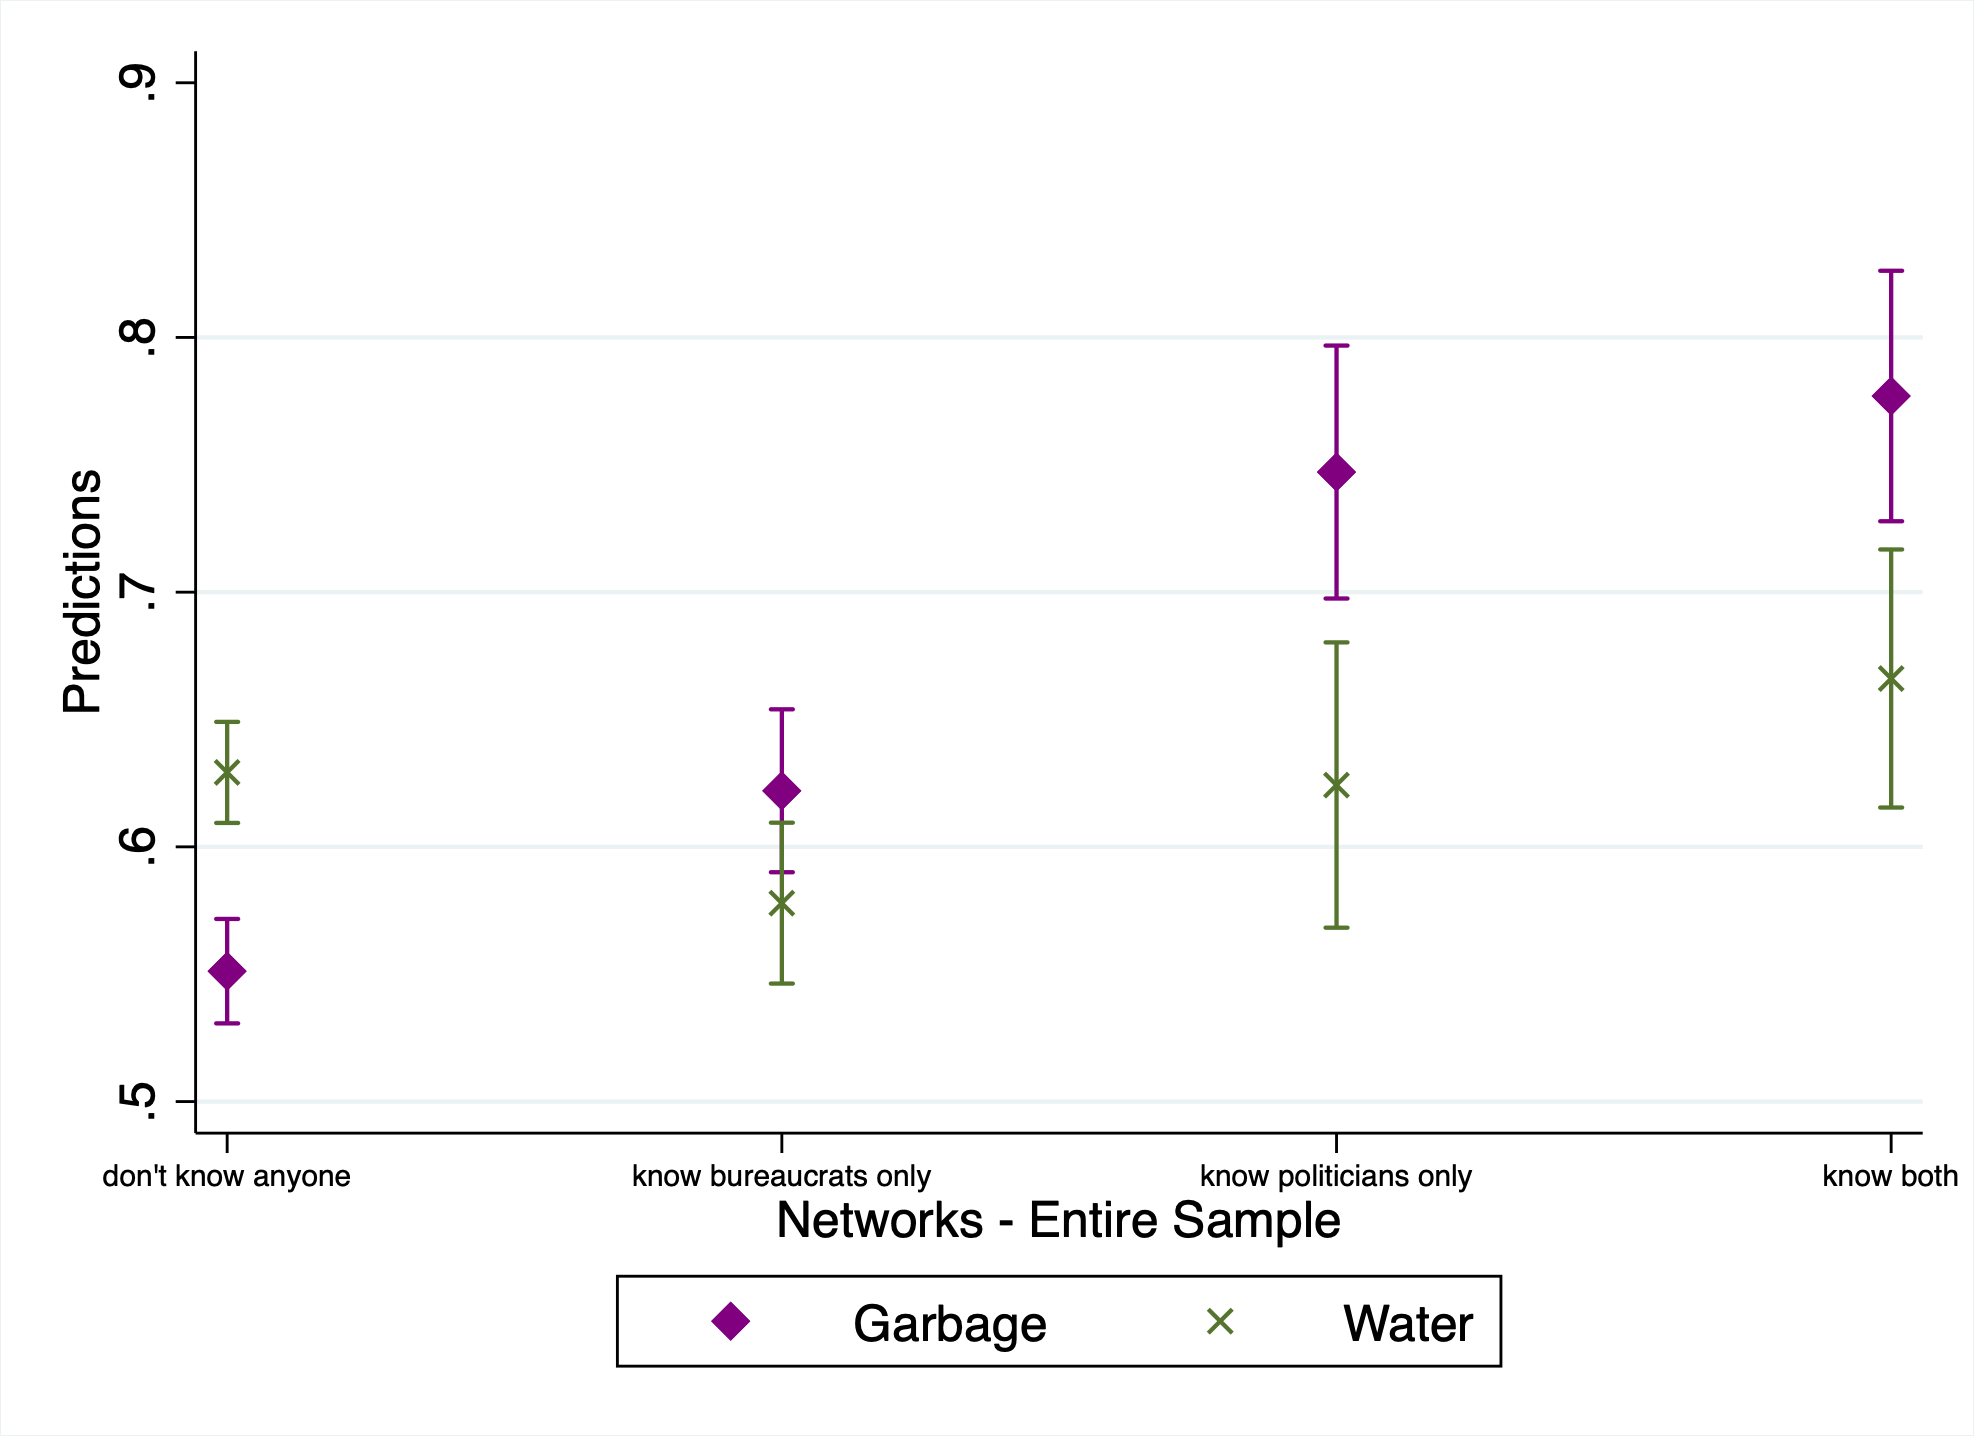
\includegraphics[scale=.4]{figures/Networks_entire sample.png}
    \caption{This figure illustrates the predicted marginal effects of network connections on access to both trash (purple diamonds) and water services (green Xs) across Bhopal and Lucknow combined. The Y-axis represents the predicted margins (the likelihood of receiving services), while the X-axis categorizes respondents based on their network connections (whether they know bureaucrats, politicians, or both). The error bars represent 95\% confidence intervals.}
    \label{fig:margins for non voting1}
\end{figure}



\begin{figure}[H]
    \centering
        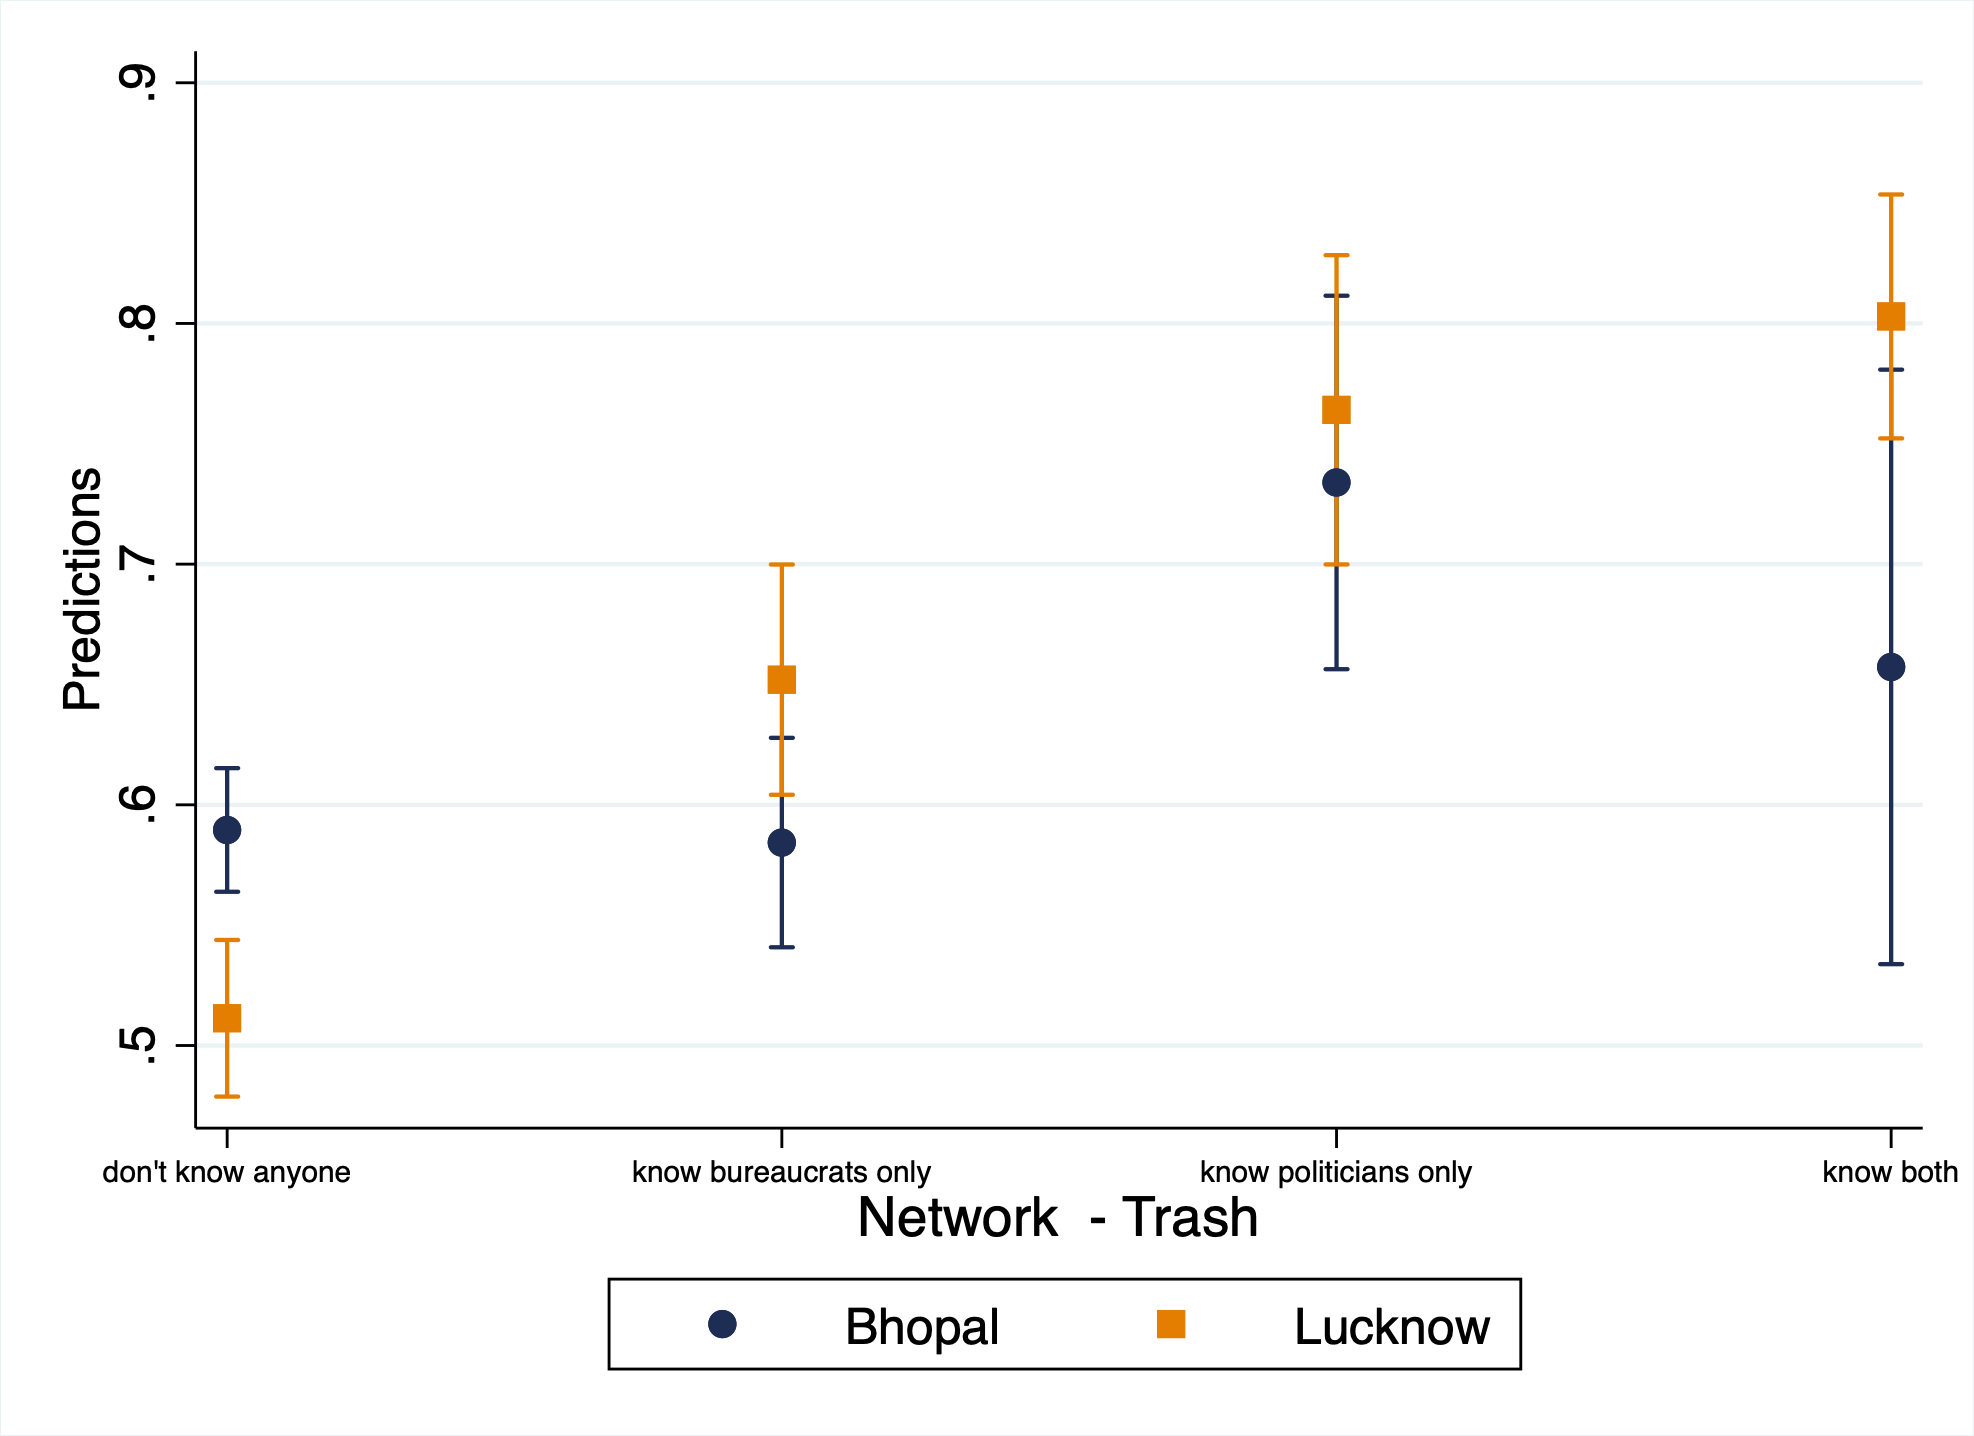
\includegraphics[scale=.4]{figures/Networks_trash.png}
    \caption{This figure illustrates the predicted marginal effects of network connections on access to trash for residents in Bhopal (blue circles) and Lucknow (orange squares). The Y-axis represents the predicted margins (likelihood of receiving trash services), while the X-axis categorizes respondents based on their network connections. The error bars represent 95\% confidence intervals.}
    \label{fig:margins for non voting}
\end{figure}

\begin{figure}[H]
    \centering
        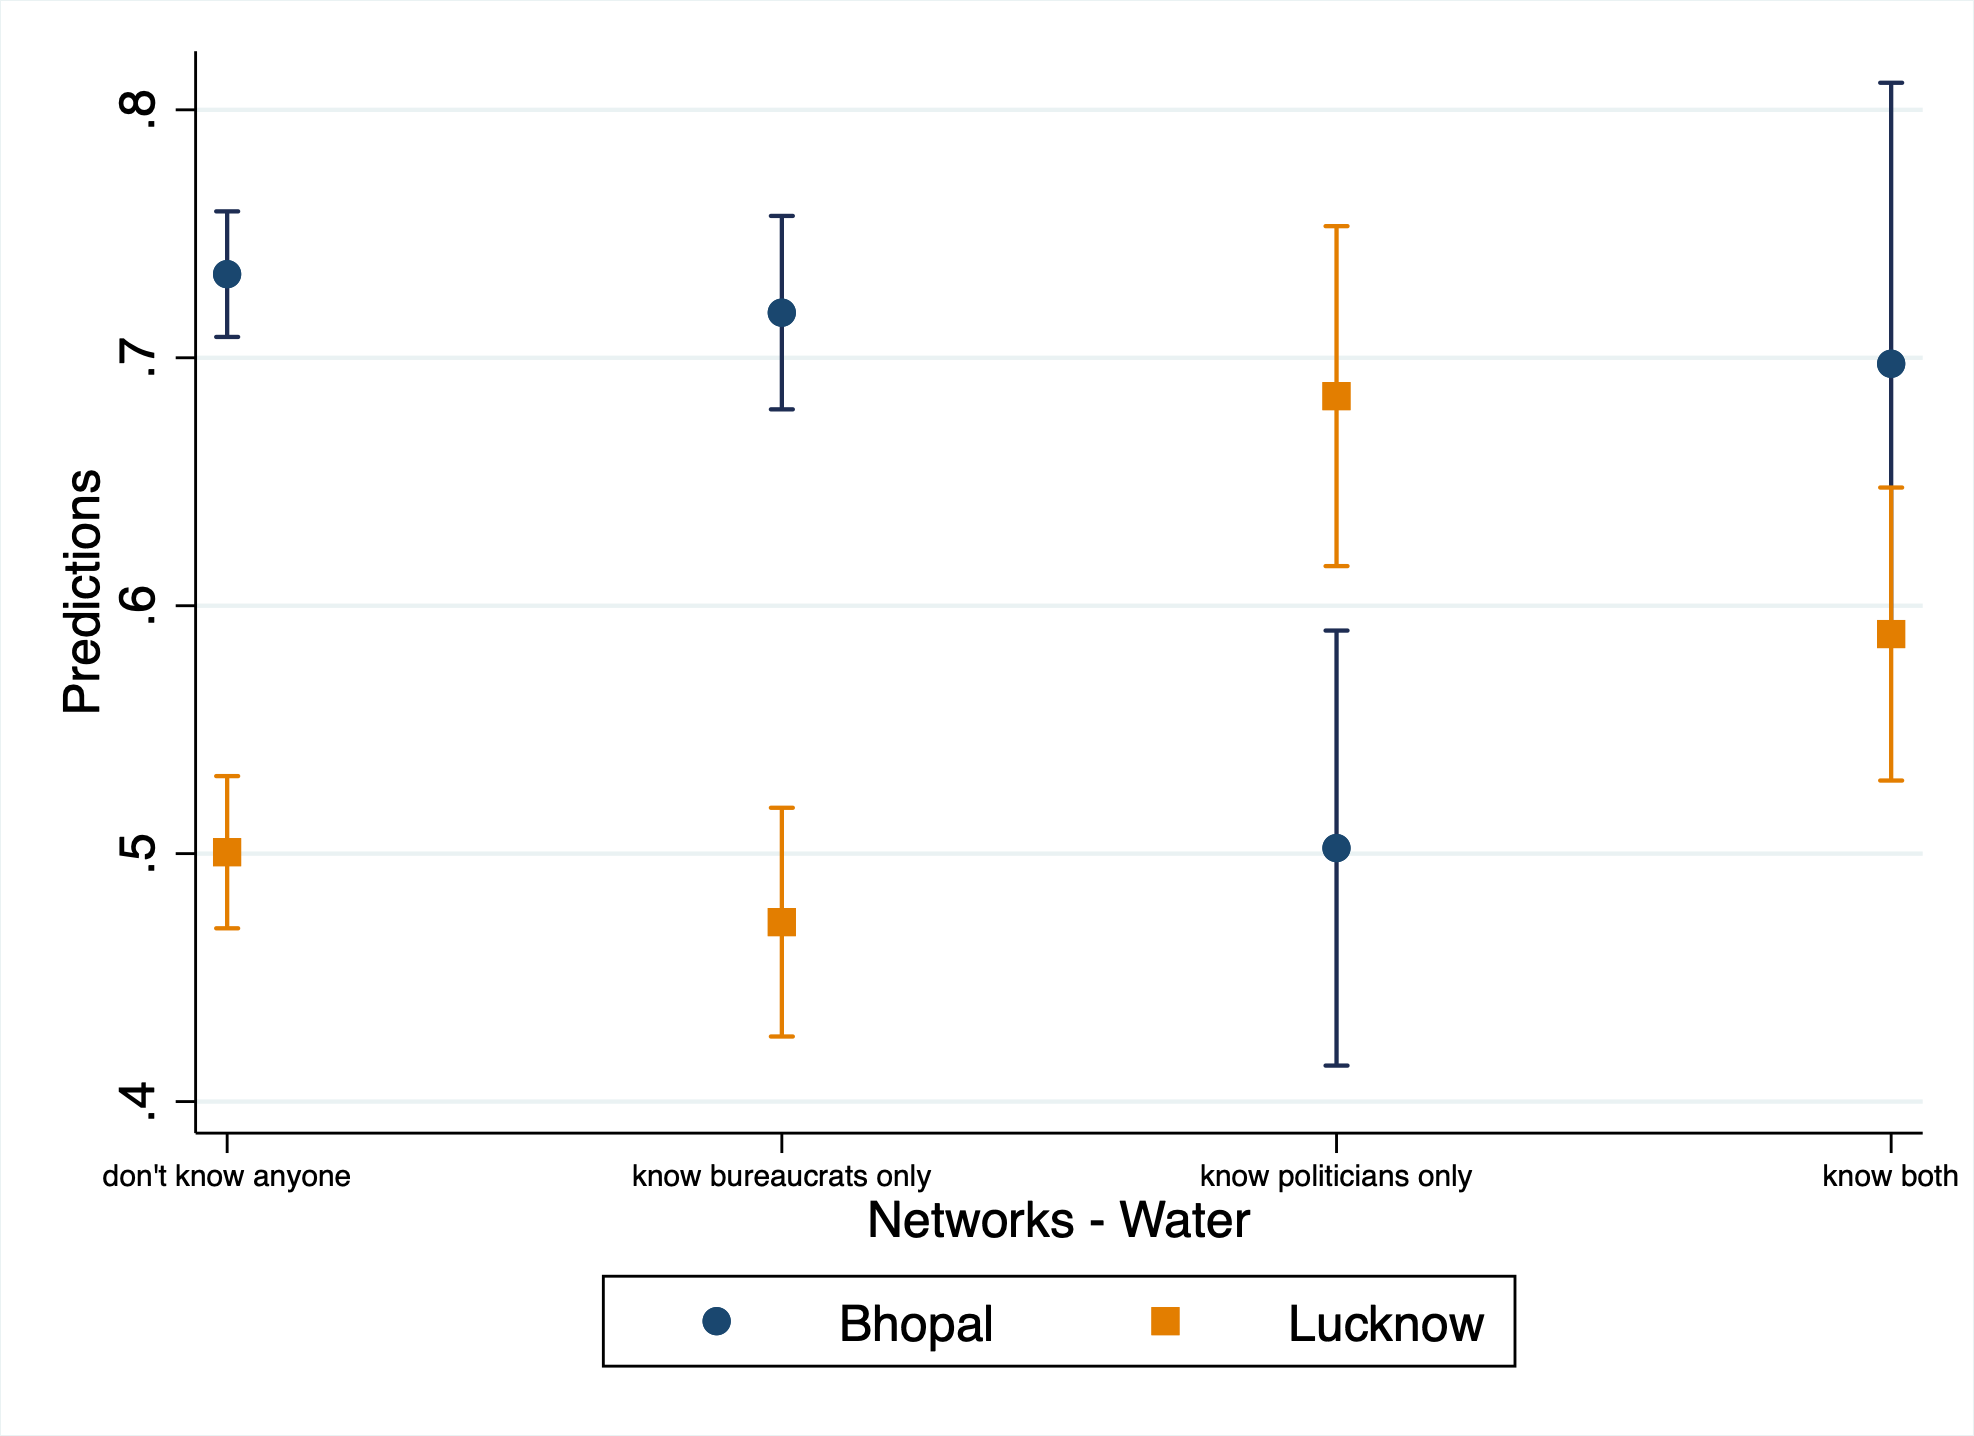
\includegraphics[scale=.4]{figures/Networks_water.png}
   \caption{This figure illustrates the predicted marginal effects of network connections on access to water services for residents in Bhopal (blue circles) and Lucknow (orange squares). The Y-axis represents the predicted margins (likelihood of receiving water services), while the X-axis categorizes respondents based on their network connections. The error bars represent 95\% confidence intervals.}
    \label{fig:margins for non voting}
\end{figure}

\begin{figure}[H]
    \centering
    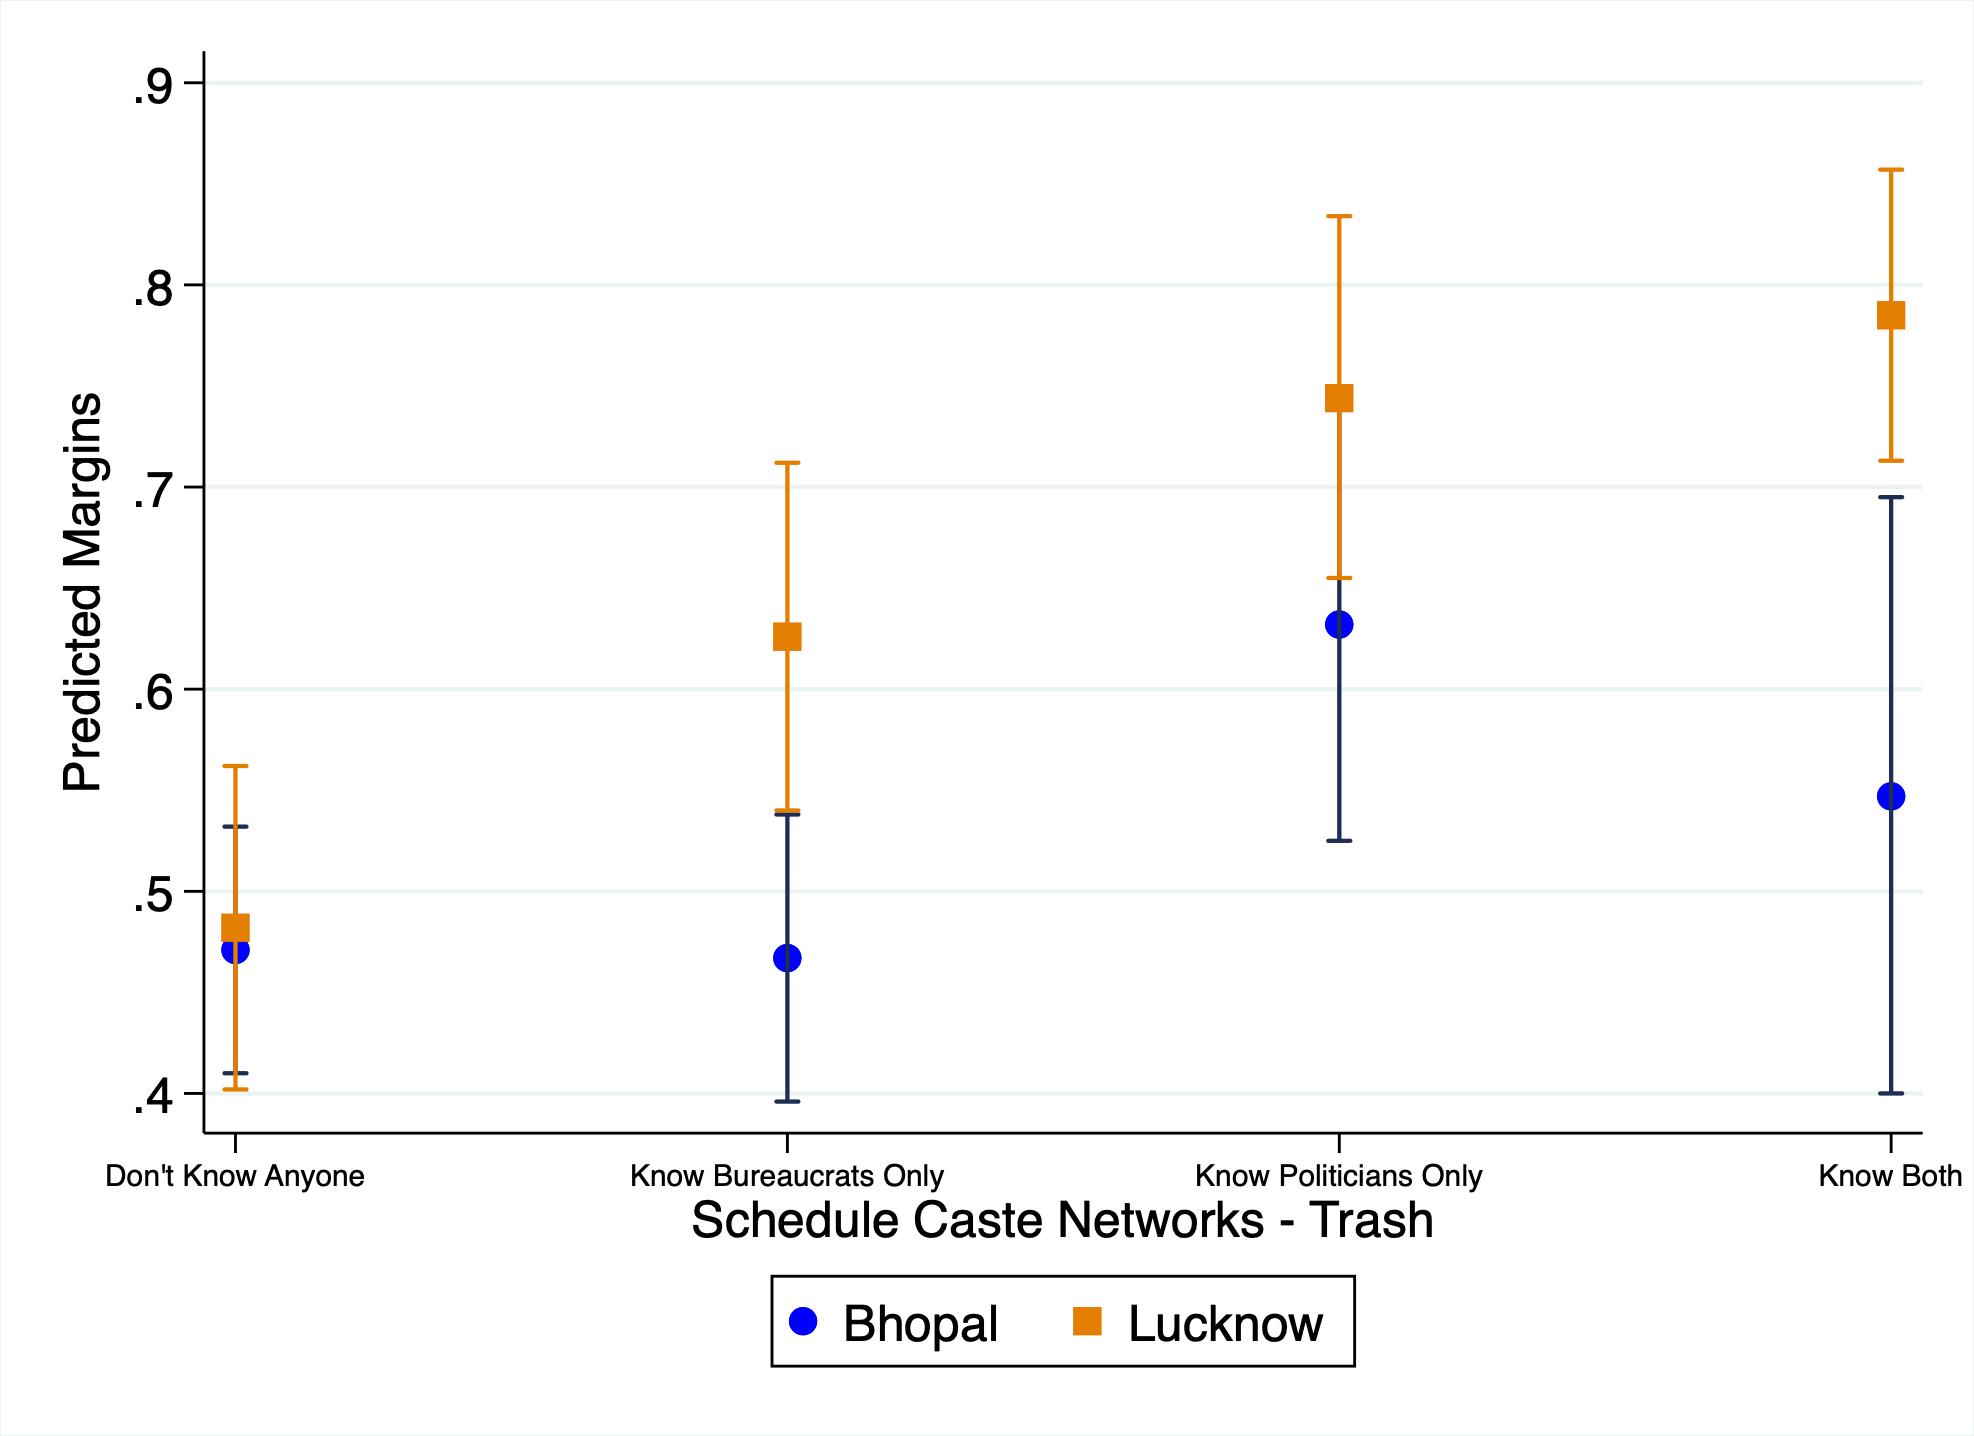
\includegraphics[scale=.4]{figures/Networks_trash_SC.png}
    \caption{SC Network - Trash: This figure displays the predicted marginal effects of different network connections (knowing bureaucrats, politicians, or both) on the likelihood of receiving trash services for Scheduled Caste (SC) residents in Bhopal (blue circles) and Lucknow (orange squares). The Y-axis represents the predicted margins (probability of receiving trash services), while the X-axis categorizes the different types of network connections. The error bars represent 95\% confidence intervals.}
    \label{fig:margins for non voting}
\end{figure}


\begin{figure}[H]
    \centering
        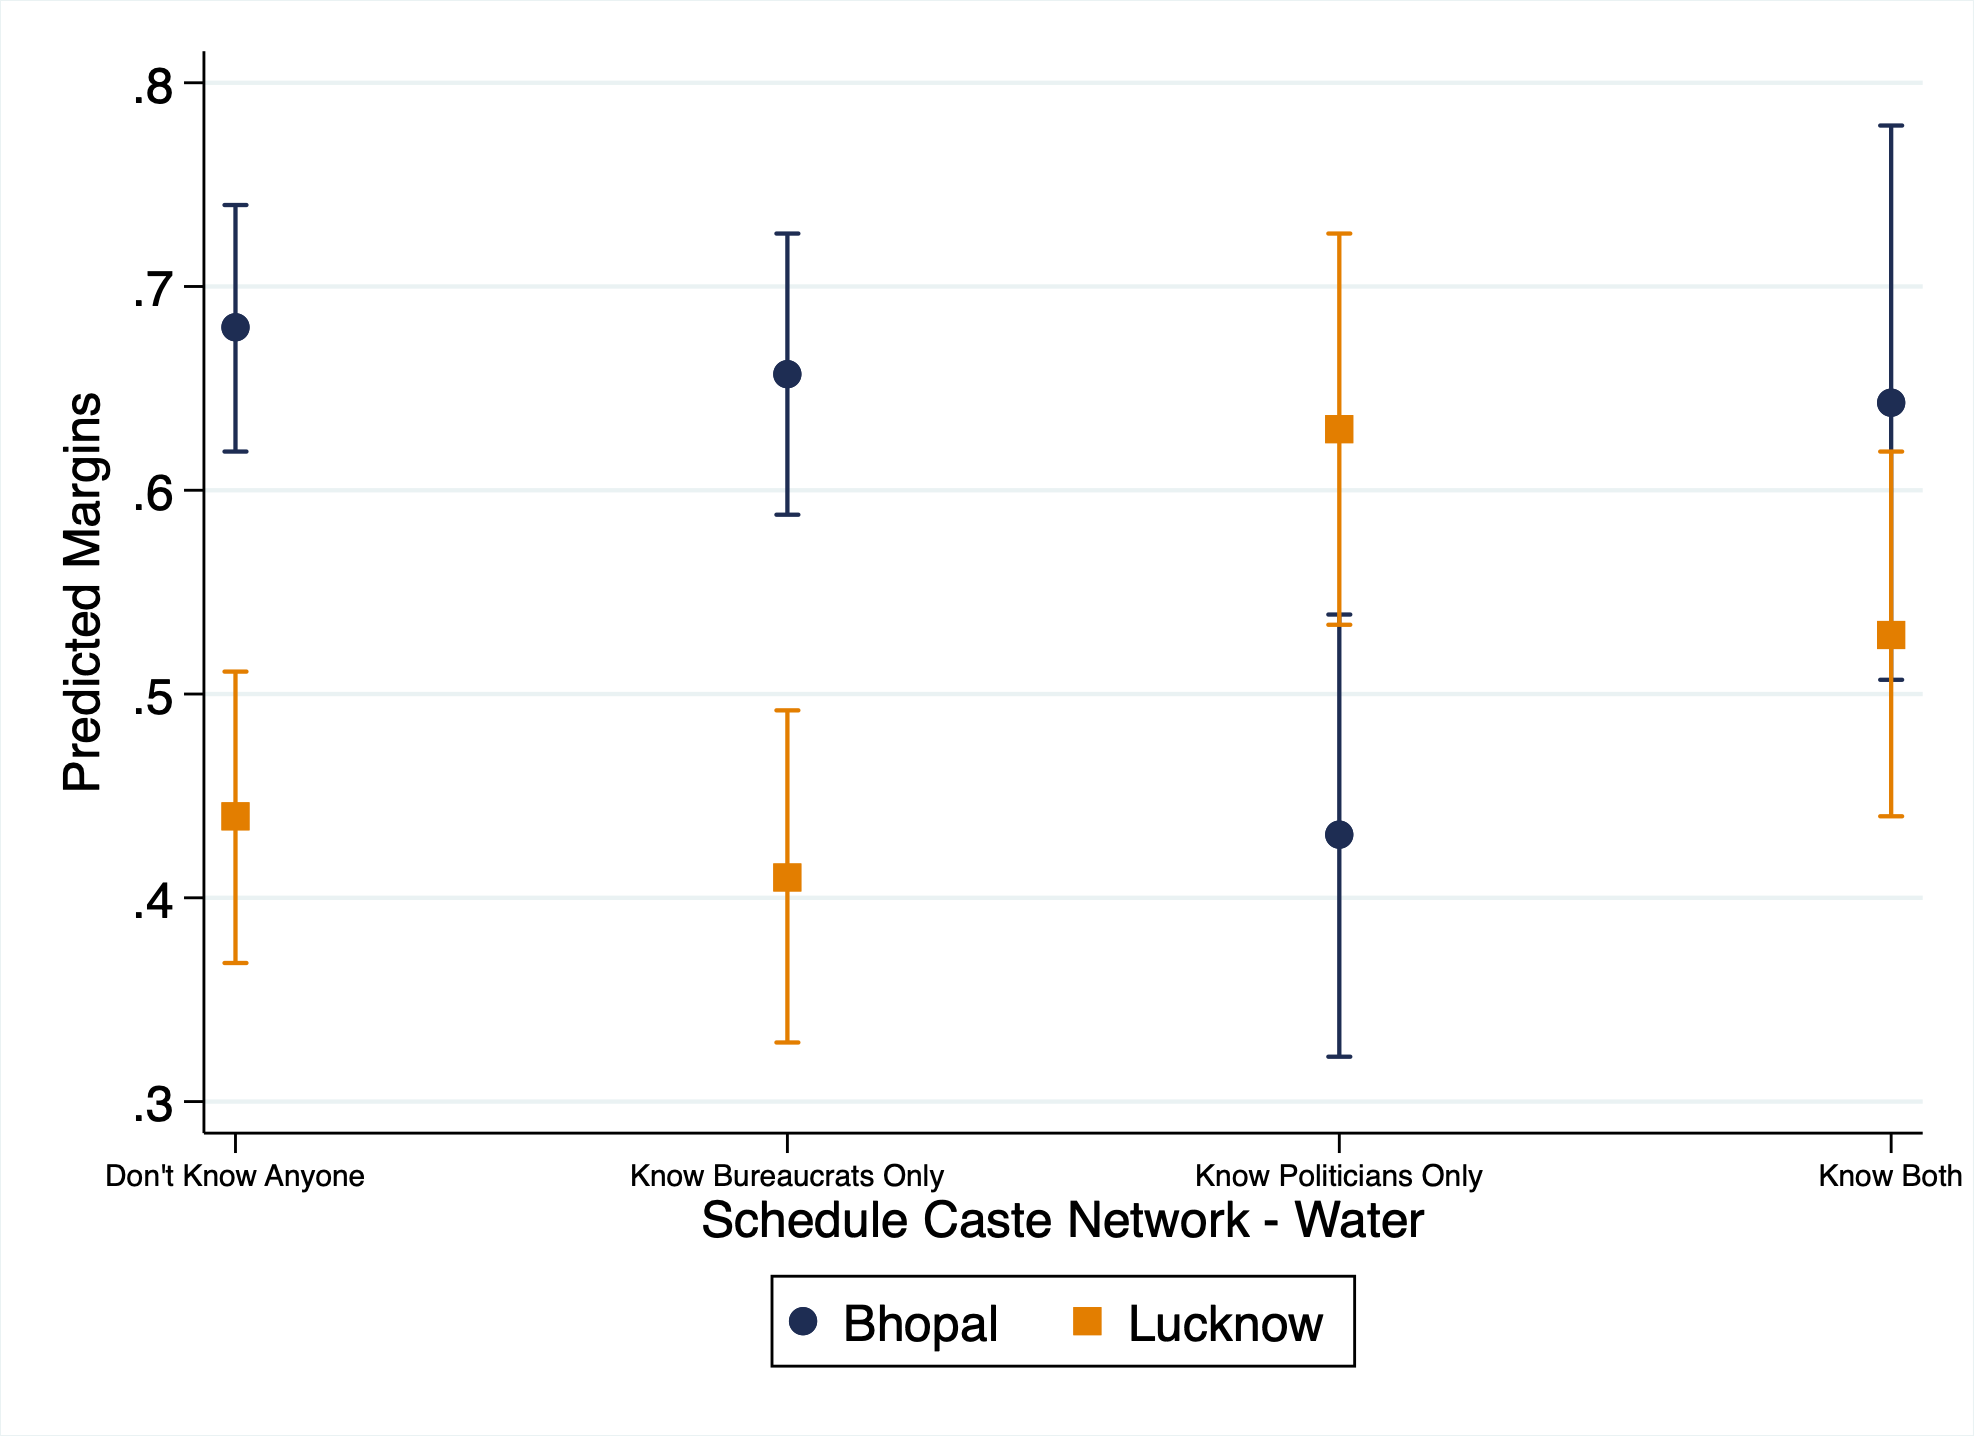
\includegraphics[scale=.4]{figures/Networks_twater_SC.png}
    \caption{ SC Networks - Water: This figure illustrates the predicted marginal effects of network connections on water service access for Scheduled Caste (SC) residents in Bhopal (blue circles) and Lucknow (orange squares). The Y-axis represents the predicted margins (probability of receiving water services), while the X-axis categorizes the different types of network connections. The error bars represent 95\% confidence intervals.}
    \label{fig:margins for non voting}
\end{figure}



\begin{figure}[H]
    \centering
    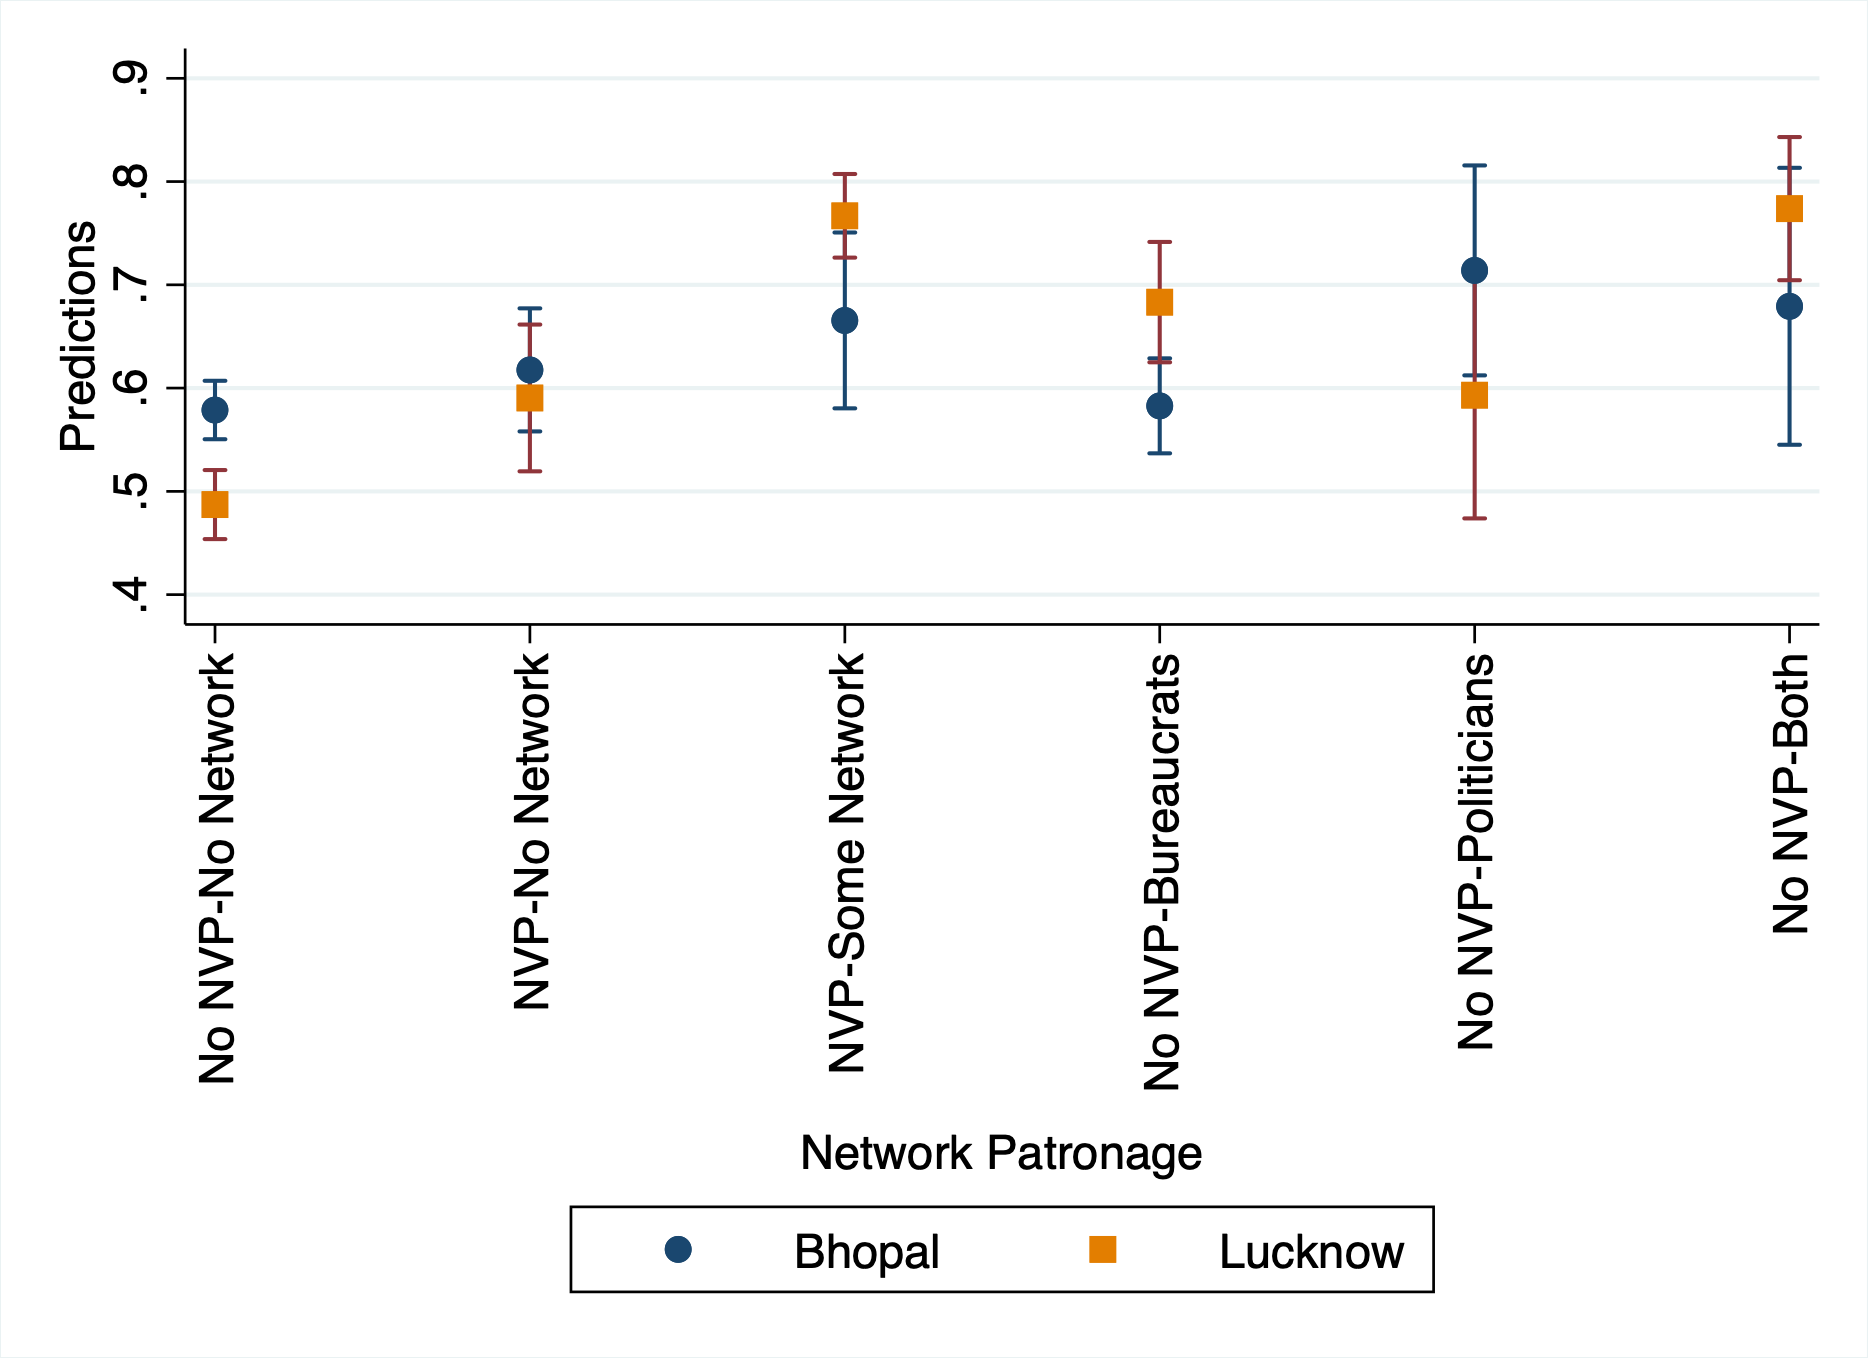
\includegraphics[scale=.4]{figures/NetPaT_garbage_.png}
    \caption{Predicted Margins of Networks and Political Participation on Trash Services: This figure shows the predicted marginal effects of different network connections (knowing bureaucrats, politicians, or both) and non-voting political participation (NVP) on trash services in Bhopal (blue circles) and Lucknow (orange squares). The Y-axis represents the probability of receiving trash services, and the X-axis categorizes: \textbf{No NVP-No Network: No participation or connections.} NVP-No Network: Political participation without connections.\textbf{NVP-Some Network: Political participation and connections.} No NVP-Both: No participation but with both bureaucratic and political connections.The error bars represent 95\% confidence intervals.}
    \label{fig:margins for non voting}
\end{figure}


\begin{figure}[H]
    \centering
        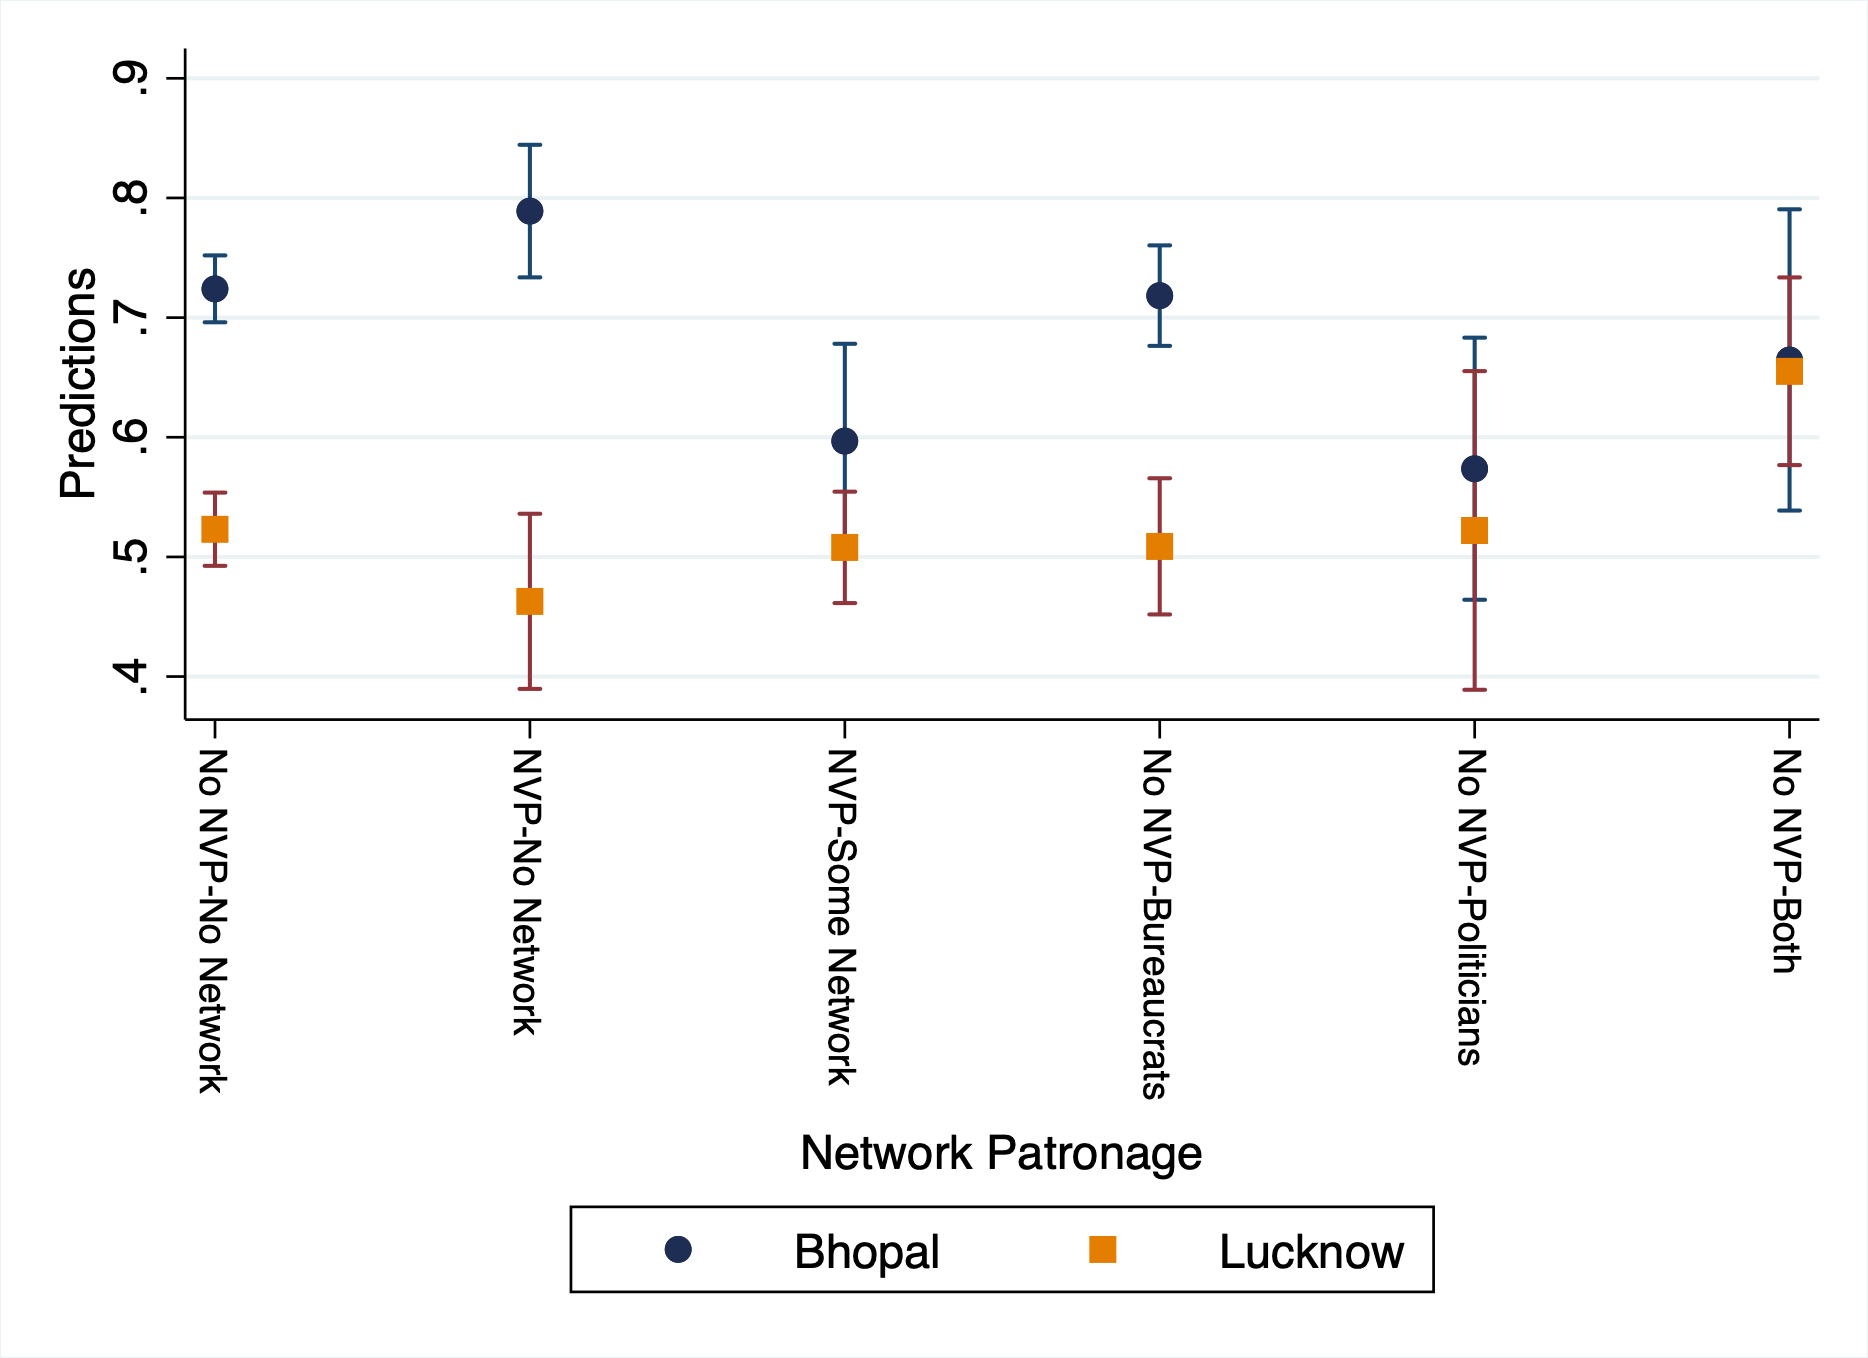
\includegraphics[scale=.4]{figures/NetPaT_water_.png}
    \caption{ Predicted Margins of Networks and Political Participation on Water Services: This figure shows the predicted marginal effects of different network connections (knowing bureaucrats, politicians, or both) and non-voting political participation (NVP) on water services in Bhopal (blue circles) and Lucknow (orange squares). The Y-axis represents the probability of receiving water services, and the X-axis categorizes: \textbf{No NVP-No Network: No participation or connections.} NVP-No Network: Political participation without connections.\textbf{NVP-Some Network: Political participation and connections.} No NVP-Both: No participation but with both bureaucratic and political connections.The error bars represent 95\% confidence intervals.}
    \label{fig:margins for non voting_2}
\end{figure}

\subsection{Taking stock}



The comparative analysis of public service delivery in Bhopal and Lucknow illuminates critical variations in institutional performance despite similar formal governance structures. The baseline disparities are substantial: Lucknow residents face 19.7\% lower odds of receiving trash services and 56.4\% lower odds of receiving adequate water services compared to Bhopal, suggesting fundamental differences in service delivery mechanisms between the cities.

In contexts of constrained institutional capacity, social networks with political and bureaucratic actors emerge as crucial determinants of service access. However, the efficacy of these networks varies systematically with service characteristics. Trash collection, being discretionary and municipally controlled, demonstrates high responsiveness to both political participation and bureaucratic-political networks. This is particularly evident in Lucknow, where densely engaged citizens (those combining political participation with official networks) see their probability of access increase from 49\% to 77\%. Notably, marginalized groups like Scheduled Caste residents can leverage these networks to increase their access probability from 50\% to 82\%, suggesting that patronage systems, paradoxically, may facilitate service access for historically excluded groups in contexts of weak institutional capacity.


Water services, however, demonstrate the limitations of network-based access to complex public goods. Even citizens with strong political engagement and extensive networks struggle to significantly improve their water access in Lucknow, where the baseline probability remains at 50\% with only marginal improvements through networks. This contrasts markedly with Bhopal's consistently high water access (73\%) independent of network effects. The infrastructure-intensive nature of water provision, requiring inter-governmental coordination and technical expertise, appears relatively impervious to individual-level interventions.


To circle back, while our theoretical framework suggests that politicians (driven by electoral accountability) and bureaucrats (focused on technical expertise and long-term stability) must collaborate for effective service delivery, the empirical evidence reveals starkly different outcomes across cities and services. Why do similar institutional contexts produce different coordination patterns? How can patronage networks successfully deliver trash services without excluding marginalized groups, yet fail to facilitate the coordination necessary for complex services like water? 

The following qualitative analysis explores these questions by examining the historical evolution of trash and water systems in both cities, seeking to understand why one system developed along patronage lines while the other became programmatic, and why patronage networks, despite their success with simpler services, fail to enable the coordination necessary for universal access to complex services.

\section{Politician-Bureaucrat Coordination - Patronage or Programmatic: Understanding the Mechanism}

\vspace{5mm}

\subsection{Water Services}
This section examines how divergent institutional arrangements in Bhopal and Lucknow led to different outcomes in water service provision, despite similar starting conditions. While both cities showed comparable levels of tap water access in 1981, 1991, and 2001, their trajectories began diverging notably after 2011, with recent citizenship surveys indicating an expanding gap in service coverage.

\begin{figure}[H]
    \centering
        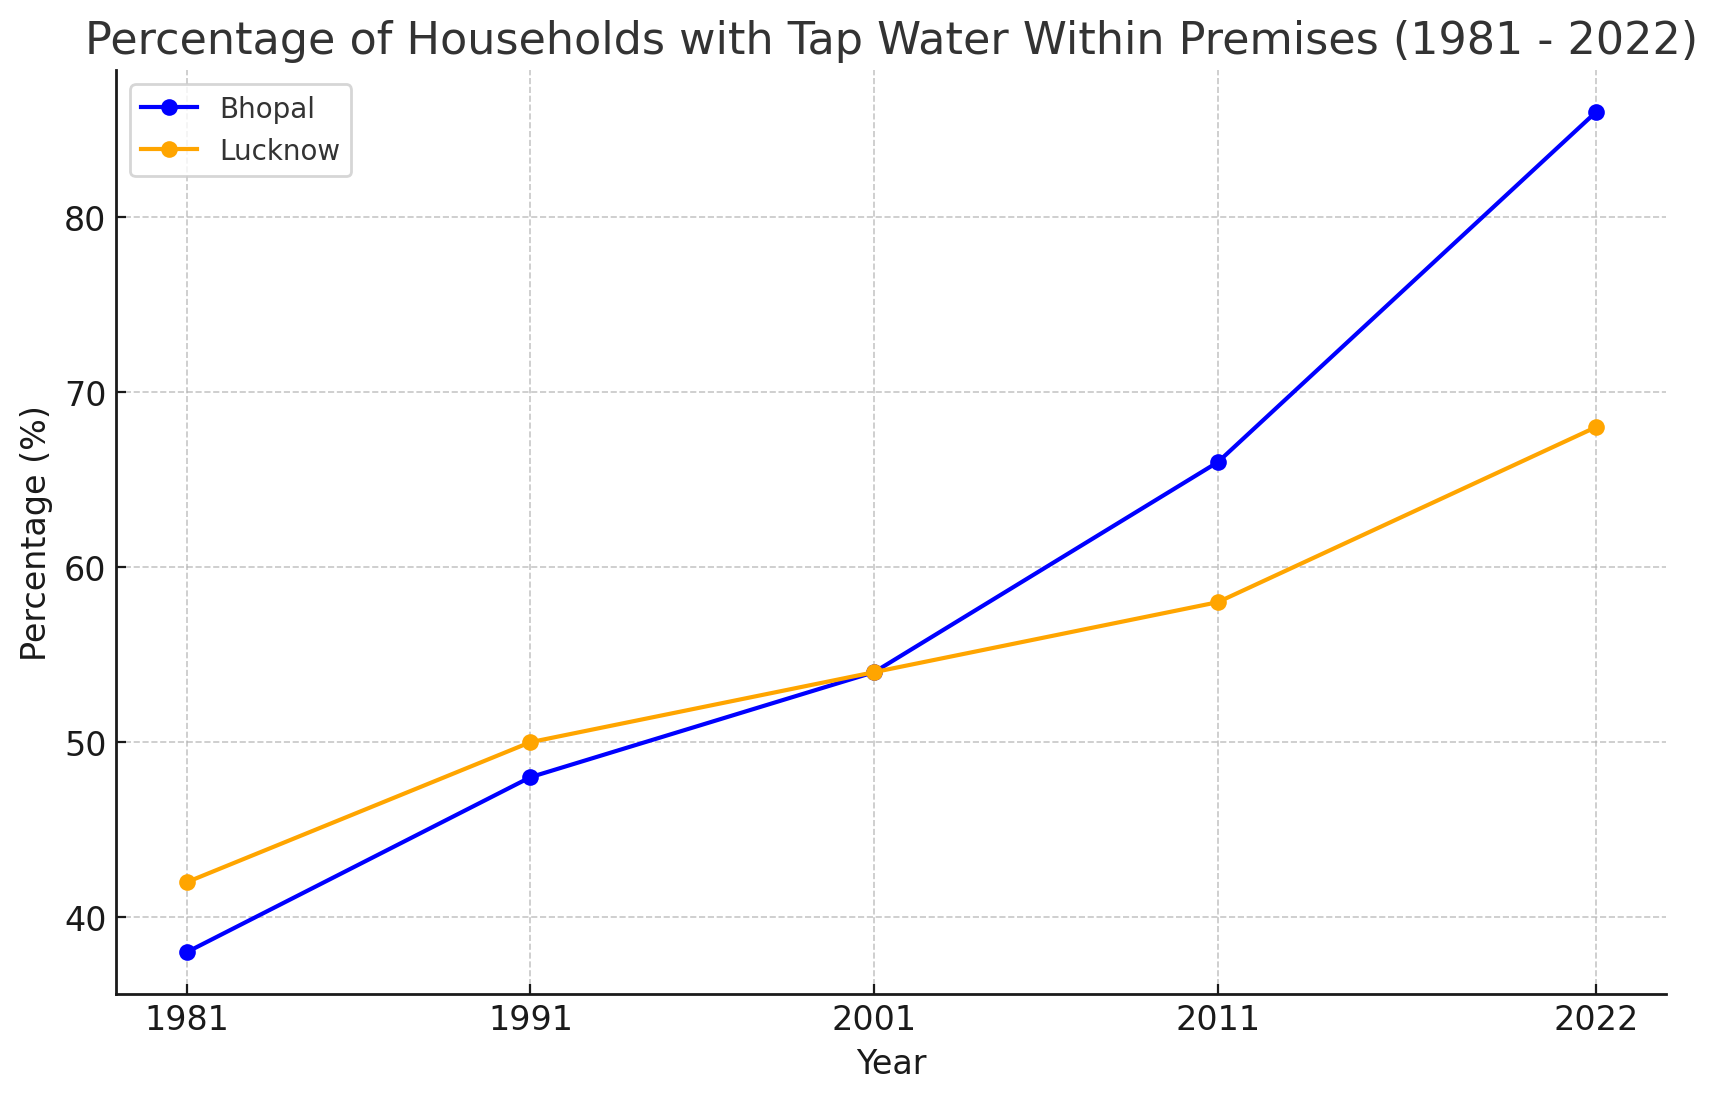
\includegraphics[scale=.65]{figures/output.png}
    \caption{Change in Tap water across Bhopal and Lucknow. Data for 1981-2011 is from the Census of India, 2022 is from Household Survey}
    \label{fig:margins for non voting_2}
\end{figure}

The introduction of India's first national urban renewal program in 2004, the Jawaharlal Nehru Urban Renewal Mission (JnNURM), provided a critical juncture for both cities. However, their institutional responses to this opportunity differed substantially, shaped by local political economies and bureaucratic arrangement

\vspace{5mm}
\textbf{Lucknow}

Lucknow's struggle with water service delivery illustrates how institutional fragmentation and competing political interests can undermine urban service provision. Despite the launch of India's first national urban renewal program (Jawaharlal Nehru Urban Renewal Mission or JnNURM) in 2004, which provided cities with both financing and incentives for universal water access, Lucknow's institutional landscape proved resistant to meaningful reform. This institutional dysfunction manifested across multiple dimensions, from political resistance to price reforms to organizational fragmentation in service delivery.

At the political level, there was a notable disconnect between local and elite politicians regarding water pricing reforms. While local politicians demonstrated some openness to revenue enhancement, acknowledging its potential to improve services through measures like the 2014 City Council's approval of "an 8\% increase in prices of water per the report of the commissioner," \footnote{Lucknow City Government meeting archives. Accessed from the Lucknow Nagar Nigam in 2021} elite politicians actively resisted such changes. This resistance was exemplified by Urban Development Minister Mohd. Azam Khan's categorical rejection of water meter installations across major UP cities \footnote{Azam Khan Opposes Water Meter Installation," \href{https://timesofindia.indiatimes.com/city/lucknow/azam-khan-opposes-water-meter-installation/articleshow/22306030.cms}{The Times of India, September 5, 2013}}. In a personal interview, the then Minister justified this position by arguing that "the funds required for such installations would have been more effectively used to improve drinking water supply in underdeveloped urban neighborhoods.\footnote{Interview with Md. Azam Khan, Minister for Urban Development 2012-2017, Rampur Jail 2022}" This stance reflected a broader political reluctance to implement pricing reforms, even when they were tied to development funding.

The institutional challenges were particularly evident in the operations of the Lucknow Jal Sansthan (LJS), established in 1975 to manage the city's water resources \footnote{The Uttar Pradesh Water Supply and Sewerage Act, 1975 (Act 43 of 1975), enacted by the Uttar Pradesh Legislature, provides the legal framework for the establishment and regulation of water supply and sewerage services in the state, including the creation of the Uttar Pradesh Jal Nigam and local Jal Sansthans to manage these services.
}. Despite its intended design as an autonomous entity, the LJS has struggled with limited financial independence, remaining heavily dependent on state grants even for basic operational expenses. This financial constraint was exacerbated by the Uttar Pradesh government's rural-centric budget allocation, which left urban water bodies with minimal resources\footnote{With 78\% of Uttar Pradesh being rural, the state's water management priorities and budget allocations heavily favored rural areas. This bias is starkly evident in the budget allocation: of the total INR 17,000 crore (\$2.014 billion) , the rural sector received 15,000 crore (\$1.778 billion), while the urban sector was allocated a mere 2,000 crore (\$0.237 billion). Uttar Pradesh Budget Analysis 2021-22," \href{https://prsindia.org/budgets/states/uttar-pradesh-budget-analysis-2021-22}{PRS Legislative Research}, accessed November 18, 2024}. Attempts to reform this structure through initiatives like merging and then re-separating urban and rural water bodies failed to address these fundamental issues, leaving the LJS in a perpetual state of financial and operational vulnerability \footnote{About Rural Jal Nigam," Uttar Pradesh Jal Nigam, accessed November 18, 2024,}. The dysfunction extended to project implementation and inter-organizational relationships. Efforts to integrate the LJS into the Lucknow Municipal Corporation (LMC) structure encountered significant resistance, with LJS employees expressing concerns about maintaining operational autonomy and service quality \footnote{Employees of Lucknow Water Department Formed a Front Against Being Absorbed in Lucknow Municipal Corporation," \href{ https://www.amritvichar.com/article/405452/employees-of-lucknow-water-department-formed-a-front-and-wrote#gsc.tab=0}{Amrit Vichar}, accessed November 18, 2024,}. The unusual reporting structure, where the LJS General Manager remained under UP Jal Nigam authority rather than city officials, created additional layers of complexity and hampered coordinated action \footnote{ Interview with Arvind Kumar Giri, Under Secretary, Uttar Pradesh. Lucknow 2022}.

What further complicated matters was the complete marginalization of LJS, the primary water service provider, in the implementation of major water projects under the union government's funding program. Instead of leveraging the institutional knowledge and expertise of LJS, the state government decided to locate the project management unit within the state's Urban Development Department \footnote{Evaluation Report: India Financial Institutions Reform and Expansion–Debt and Infrastructure Ex-Post Evaluation, WASH Ex-Post Evaluation Series—Water Communications and Knowledge Management (CKM) Project, September 2018, 11, 13}. This decision not only reflected a deep distrust of city-level institutions but effectively sidelined the very organization meant to provide water services \footnote{Interview with PK Srivastava, Additional Municipal Commissioner LMC 2009-2013, Lucknow 2022
}. Elite bureaucrats at the state secretariat, wary of potential political-contractor nexus at the city level, deliberately kept both city politicians and bureaucrats at arm's length from the project implementation\footnote{ibid.}\footnote{Interview with MG Ramachandaran, Urban Development Secretary 2004-2009, Government of India. Delhi 2023}. However, this attempt to centralize control paradoxically led to a situation where those most familiar with the city's water infrastructure and needs - the LJS officials - were excluded from critical decision-making processes\footnote{Final City Water Plan for Lucknow, 2011}.\footnote{Interview with SK Singh, PCS officer, Head of Lucknow Jal Sanshthan 2007-2012. Delhi 2023
}

The resulting vacuum in local expertise became evident in project implementation. With the LJS marginalized and city government stripped of meaningful policy-making power, state-level bureaucrats found themselves having to arbitrate between competing interests without adequate ground-level understanding. The critical decision of where to initially implement the water project - whether to attempt city-wide coverage or focus on the older areas that formed the core of the city government's political base - became a contentious issue precisely because those making the decisions lacked the local context that LJS could have provided.
The site selection process for water projects became particularly contentious, exposing these institutional fault lines. While DFID and the Urban Development Department prioritized newly incorporated areas like Gomti Nagar and Transport Nagar, the Lucknow Municipal Corporation advocated for older, central neighborhoods, reflecting local political interests\footnote{International Financial Institutions as part of the reform to fund projects. In Bhopal, ADB and the UK's Department for International Development (DFID) were active in urban projects. Meanwhile, in Uttar Pradesh, USAID's FIRE-D project worked on urban reforms. These IFIs promoted city development plans, market-based infrastructure financing, and capacity building reforms. In the case of Lucknow, FIRE-D USAID were responsible, and while  the major funding went to water related projects}. This disagreement was further complicated by disputes over contractor selection, where political affiliations played a significant role. The state's ruling Samajwadi Party favored Emaar Construction Limited, a Dubai-based firm, while the BJP-controlled LMC preferred a local bidder \footnote{Interview with Kaushal Shankar Pandey (INC) , councilor from Aliganj ward. Lucknow 2022
} \footnote{Interview with Md. Saifullah, Councillor for the Yadunath Sanyal ward from 2006-2017, Lucknow 2022}. These conflicts ultimately led to DFID's withdrawal from the project, as they feared both contract violations and the potential precedent this might set for future collaborations \footnote{Interview with RK Srinivasan, USAID Water, Sanitation and Hygiene Finance (WASH-FIN) Delhi 2023
}. While the Asian Development Bank chose to continue their involvement, they significantly reduced their financial commitment by half. \footnote{Office of the Principal Accountant General (General & Social Sector Audit), Uttar Pradesh. (2016). Annual Technical Inspection Report on Urban Local Bodies for the Year Ended 31 March 2016 (p. 23, 24)}

The city's experience with water project implementation underscores a critical insight about urban governance: even when funding is available, institutional fragmentation can severely impair project execution. DFID officials repeatedly advised elite bureaucrats in the state Secretariat that municipal management would enhance project effectiveness, but these recommendations were largely ignored. After two years of limited progress and unresolved disagreements over key issues, DFID's decision to exit the project entirely reflected the severity of these institutional challenges\footnote{Interview with RK Srinivasan, USAID Water, Sanitation and Hygiene Finance (WASH-FIN) Delhi 2023}.

\vspace{5mm}
\textbf{Bhopal}

Bhopal faced similar pressures regarding water charges, with both elite and city politicians initially resistant to reforms. However, the city's approach to implementing the union government's water program differed significantly from Lucknow's, largely due to its constrained financial position \footnote{Interview with Deepti Gaur Mukherjee, Indian Administrative Services, Commissioner Bhopal Municipal Corporation, 2009-2011. Bhopal 2022}. While both cities were starved for money, Lucknow, as a constituency of a former prime minister, believed it could secure funding through alternative political channels\footnote{Interview with SK Shastri, Officer on Special Duty to A.B. Vajpayee, Prime Minister of India (2009-2014) and three time member of Parliament from Lucknow. Delhi 2023}. Bhopal held no such primacy, forcing a more pragmatic approach. As one consultant noted, "Cities in Madhya Pradesh were not pushovers. The Mayors knew they were powerful and maintained independence from the state leadership."\footnote{Interview with Arkaja Singh, a private consultant with experience working with various International Financial Institutions and was a consultant hired by DFID for UDAY. Delhi 2022
} Unlike Lucknow, where decision-making shifted to the secretariat, Bhopal's institutional actors recognized that the union government's plan represented their only viable path forward for improving water services, creating pressure for internal alignment between state and city institutions \footnote{Interview with Deepti Gaur Mukherjee, Indian Administrative Services, Commissioner Bhopal Municipal Corporation, 2009-2011. Bhopal 2022}.

A crucial difference emerged in how the Project Management Unit (PMU) for the water projects in the 2000s was positioned and operated. While both cities received support from ADB and DFID for establishing PMUs, Bhopal's unit was situated within the city government (Bhopal Municipal Corporation or BMC) rather than at the state level\footnote{Interview with Priyanka Das, Indian Administrative Services, Madhya Pradesh Cadre. Bhopal 2022}. This positioning proved critical as it enabled direct collaboration with the state level bureaucracy - officers from the Madhya Pradesh Municipal Administration Services, a cadre dedicated exclusively to urban administration\footnote{nterview with Neelesh Dubey, Madhya Pradesh Municipal Administrative Services. Bhopal 2022
}. These career bureaucrats, operating under the City Commissioner's authority, brought crucial urban expertise to project implementation \footnote{Madhya Pradesh Urban Services for the Poor (MPUSP) Project. (2012). Project completion review: Madhya Pradesh Urban Services for the Poor (MPUSP) Project. Retrieved from https://iati.fcdo.gov.uk/iati_documents/3780260.odt.}.

The effectiveness of this arrangement was highlighted by Bruce Pollock,  head of the DFID project for Madhya Pradesh. He particularly emphasized the role of these officers, noting that "they were really the core of the program in Bhopal, whose negotiating skills - got the work done." Explaining further the unique value these state-appointed bureaucrats brought: "These guys had been trained in the PMU to understand the legalistic aspects of contracts but they added their knowledge of the local landscape. They identified builders, who had political connections or politicians open to contract negotiations. This could not have been done either by us (meaning the international agency) or the Commissioners (elite IAS officers)." \footnote{Interview with Bruce Pollock, who headed the DFID program in Madhya Pradesh from 2008 to 2013. As one observer noted, "These officers moved from one city to another but were retained in the PIU, so we knew we could rely on training a select group of officers which, even if transferred, would remain part of the system.” Zoom 2021, 2022,2024.
}

The implementation of the \$28 million ADB/DFID-funded water project in 2007 illustrates how Bhopal's institutional arrangement facilitated effective navigation of competing interests. The project faced multiple stakeholder demands: politicians sought coverage for their areas and contracts for associates, ADB/DFID pushed for equitable network distribution, and bureaucrats, particularly engineers, had their own interests in contracts and licenses\footnote{ibid.}. Rather than allowing these competing interests to paralyze implementation, Bhopal's state level bureaucracy became a key player in making the program operational\footnote{Project Uday. (n.d.). Project management. Retrieved from https://web.archive.org/web/20180828214026/http://projectuday.gov.in/ProjectMgt.htm}.

The then Mayor of Bhopal, Sunil Sood, explained that local contractors were a vital part of the process and an essential component of the political ecosystem. While elite IAS officers were aware of these dynamics, they were reluctant to engage directly.\footnote{nterview with Sunil Sood, Congress led Mayor of Bhopal City Government (2004-2009), Leader of Bhopal City Council (2000-2004),, City Councillor (1995-2009) } As Manish Singh, the then IAS officer posted as Commissioner of BMC, explained, "You can understand the implications of getting these contractors in the office. Negotiating is not my job, but I did ask my deputies to look into this – they knew the landscape better. The guidelines were clear; either get it passed in the house or surrender the project, so s\textit{omeone had to do the dirty job}."\footnote{Interview with Manish Singh, Indian Administrative Services, Madhya Pradesh Cadre. Bhopal 2022
}

The resolution came through the joint efforts of state level bureaucracy and politicians. Abhay Ranjan Gowankar (then Assistant Commissioner, Administration in the BMC) and Devinder Chauhan (current Officer on Special Duty to Minister of Urban Development, Madhya Pradesh and then Deputy Project Coordinator of JnNURM) worked with Mayor Sunil Sood to find middle ground, making the project compatible with local realities. This involved assisting local contractors in meeting technical bid requirements and organizing meetings with stakeholders, including Louis Berger, one of the three international firms being considered for the water tender.\footnote{Throughout this research, I conducted interviews with a diverse range of stakeholders, and certain names repeatedly emerged as influential figures. This recurring mention was triangulated through official records, including meeting minutes from the Municipal Corporation, reports from third-party entities such as DFID, and input from government officials and political party representatives. Additionally, independent citizens actively engaged in local affairs provided further assessment and context. While these observations are based on interviews conducted with various stakeholders, the frequent mention of specific officers’ names underscores their significant role in local governance discussions during this period.}

Over multiple meetings, which stakeholders referred to as aligning "vision," state bureaucrats helped contractors and politicians devise implementation strategies.\footnote{Interview with Vivek Aggarwal, Louis Berger Limited. Delhi, 2023.
} They broke the project into smaller "packages" - manageable components like pipelines, road drains, culverts, or constructing local offices - making local contractors eligible for participation.\footnote{Iterview with Vijay Datta, JnNURM incharge, Urban Development and Housing Department, Madhya Pradesh Government, Bhopal, 2023.
}The bureaucrats also mediated with engineers to "reduce" bribes from contractors (referred to as cut money), recognizing the contractors' need to invest in better human and tech resources.\footnote{Interview with Devendra Chauhan, Madhya Pradesh Municipal Administrative Services, who was then with the BMC and is now an Officer on Special Duty (OSD) to the Minister of Urban Development. Bhopal 2023}\footnote{nterview with Arkaja Singh, a private consultant with experience working with various International Financial Institutions and was a consultant hired by DFID for UDAY. Delhi 2022
} Politicians, in turn, reassured councillors by ensuring their contractors were included in other projects like the water tender.

This pragmatic approach continued into recent times. In 2022, during the implementation of AMRUT 2 (JnNURM's successor) projects for dumpsite cleaning and housing construction, similar negotiations occurred between contractors and the Mayor in Council members. Being present in these discussions, some of them focused on organization, others explicitly addressed the distribution of illicit payments across bureaucratic and political networks.

\vspace{5mm}
\textbf{To summarise: }
The contrasting experiences of these cities illuminate two distinct patterns of politician-bureaucratic  coordination. In Lucknow, while city-level bureaucrats and politicians maintained their own coordination mechanisms, they failed to effectively navigate multiple levels of the state apparatus. The isolation of the LJS's expertise, combined with the state-level bureaucracy's attempts to bypass local actors, created insurmountable coordination failures. Even when local political consensus emerged, as with the 2014 water price increase approval, the inability to bridge different levels of state authority ultimately paralyzed implementation.

In Bhopal, state-level bureaucrats emerged as crucial intermediaries, operating both within and beyond state boundaries. Their role transcended conventional bureaucratic functions, as they actively built bridges between different levels of state authority while simultaneously engaging with the local business community. This dual capacity for internal coordination (navigating between elite IAS officers, political leadership, and street-level bureaucrats) and external intermediation (working with contractors, managing political pressures, and maintaining project integrity) proved essential for translating programmatic policies into implementable reality. 

\subsection{Trash Services}

\vspace{5mm}
\textbf{Lucknow} 

In Lucknow, the nature of municipal solid waste management reveals how fragmented political representation and bureaucratic arrangements can create a system of "selective inclusion" that paradoxically undermines effective service delivery. At the core of this dynamic is the concentration of marginalized group representation solely at the municipal level, making garbage management—as both a major employer and essential service—a critical tool for political patronage.

The municipal administration became a prime target for political parties' patronage strategies, particularly in sanitation work. Nearly 60\% of all municipal appointments in the past decade were made through direct political intervention, with sanitation workers forming the largest category. This institutional capture was particularly evident in the city's bottom-heavy staff structure, where 5,745 out of 7,200 employees were sanitation workers. These positions, requiring minimal qualifications (just primary school education) and no formal interviews, became valuable political currency.\footnote{Lucknow continues to suffer from a lack of consistent statistical information on employment. Various reports from within the city government, the union government, newspaper clippings, and audit reports have quoted differing numbers. These discrepancies necessitated triangulating these figures to provide the most accurate possible estimate.
The Comptroller and Auditor General in its reports have pointed “The status of Safai karmchari during 2005 and 2006 was not made available to the audit even in 2011” pg. 30 link: https://cag.gov.in/uploads/download_audit_report/2011/Uttar_Pradesh_City_6_2011_chap_5.pdf 
}

This aligns with and extends beyond Chandra’s (2004) concept of
”patronage democracy.” In Lucknow, identity-based political parties such as the Bahujan
Samaj Party (BSP) and Samajwadi Party (SP) transformed SCs’ access to public services,
particularly through their control of the Lucknow Municipal Corporation (LMC).\footnote{For a detailed examination of the relationship between jobs and ethnic parties, Kanchan Chandra’s "Why Ethnic Parties Succeed"  On page 85, Chandra explores how these parties leverage employment opportunities to build loyalty and support, offering a critical analysis of the political dynamics involved.
} Through
an ethnography and comparative historical analysis, my research reveals the mechanism
behind this change. These parties leveraged their control over the Lucknow Municipal
Corporation (LMC) to create a robust patronage network, particularly in the sanitation
sector.\footnote{Interview with Dr. P. K. Trivedi & Dr. Shikha Singh, Giri Institute of Development Studies, Lucknow, 2022. Also read: "When Neo-liberal Agenda Negotiates Dalit Agenda: The Case of BSP in Uttar Pradesh," in Trivedi, P. K. (Ed.), The Globalization Turbulence: Emerging Tensions in Indian Society (pp. 268-288). Rawat Publications.
} By strategically positioning members of SC communities within the LMC, especially in sanitation roles, parties like BSP and SP have created pathways for these groups
to access better services. This is evidenced by specific policy actions, such as the SP government’s 2013 initiative targeting the Valmiki community with 40,000 new sanitation worker
positions and improved wages.\footnote{Before elections, all parties make promises to Dalit groups to offer jobs in these positions. Indian Express. (2022, February 4). SP promises 40,000 jobs, hike in daily wage. Retrieved from https://indianexpress.com/article/cities/lucknow/sp-promises-40000-jobs-hike-in-daily-wage/
}These targeted efforts demonstrate how identity-based
political parties have actively worked to improve the lives of marginalized communities
through patronage networks and strategic placement of SC individuals in key positions
within the local government. The structure of the LMC made it an ideal vehicle for political capture, with 80\% of its workforce (5,745 out of 7,200 employees) employed as sanitation workers, many with minimal qualifications.\footnote{ Final City Sanitation Plan for Lucknow, 2011 pg. XX
}

The state-level bureaucracy in Lucknow, rather than counterbalancing these patronage pressures, became deeply embedded in them. Unlike other capital cities where IAS officers typically serve as Commissioners, Lucknow's leadership has mainly been under PCS (Provincial Civil Service) officers. From 1999 to 2024, the city saw 29 commissioners, with 24 having average tenures of just six months. These state bureaucrats, confined to state postings and dependent on political patronage for career advancement, often bypassed formal authority structures through direct political connections. 

The privatization of garbage management, rather than reforming this system, inadvertently reinforced it.\footnote{Lucknow privatized its garbage management in 2010 - after which it hired two concessionaires, all of whose contracts were terminated before time} The contract awarded to three private firms owned by a prominent local contractors with established connections to the bureaucracy and politicians—exemplified how privatization became entangled with existing patronage networks.\footnote{The audit conducted by the Auditor General of Uttar Pradesh noted:
“In NN Lucknow, records for 55 wards out of total 110, where collection of MSW was being done by the concessionaire, were not available. Thus, the audit could not verify whether the specified system was implemented in the ULBs [urban local body] for collection of waste on a regular basis… It was also noticed that NN Lucknow was not maintaining records regarding collection of user charges (details of wards, number of houses, number of bills issued, amount due and recovered as user charges). In absence of these records, the amount of due and recovered as user charges could not be ascertained by Audit. 
Office of the Principal Accountant General (General & Social Sector Audit), Uttar Pradesh. (2016). Annual Technical Inspection Report on Urban Local Bodies for the Year Ended 31 March 2016 (p. 23, 24). Government of Uttar Pradesh. Retrieved from https://agup.nic.in/pag/en/docs/ULB_English.pdf
} As the then Lucknow City Commissioner revealed: "We were stuck from both ends. Politicians here wanted to preserve subcontracting, and pressure from Delhi and Secretariat was to reform or give up any funding. There was no capacity with us - every drop of diesel had '\textit{neta ka hastakshar}' (politician's signature) and '\textit{babu ka thapa}' (a bureaucrat's stamp of approval)."\footnote{Interview with SK Singh, PCS officer, Commissioner of Lucknow 2007-2012. Delhi 2023
}

The result was a bifurcated system where private concessionaires operated in only 55 of 110 wards, while the remaining areas were serviced by firms closely tied to local councilors and lower-level bureaucracy. This arrangement became formally institutionalized in 2023, with three zones allocated to "contractors" (effectively politician-bureaucrat run firms) and five to private concessionaires.\footnote{Indi Newsline. (n.d.). Two ways of cleaning and garbage in Lucknow. Indi Newsline. Retrieved August 6, 2024, from https://www.indinewsline.com/two-ways-of-cleaning-and-garbage-in-lucknow/
} This created what one official termed a "shadow state" where formal privatization masked continued patronage-based service delivery.

The implications for service delivery were profound. While no social group was entirely excluded from services, access often depended on political connections.\footnote{Indian Express. (2022, March 20). Lucknow mayor wants EOW to probe corruption by civic officials. Indian Express. https://indianexpress.com/article/cities/lucknow/lucknow-mayor-wants-eow-to-probe-corruption-by-civic-officials-6533614/
}\footnote{Similar case existed in my second field site of Aliganj where a tax officer used his connection with the senior bureaucrats to continue working in the city government in spite of suspension order issues. I can include the case if required. 
}As one councilor explained, "Corporation never had funds to clean the city - neither then, nor now. If I do not employ my people to collect garbage, my support will wane. If I don't do it, garbage will not be lifted." \footnote{Interview with Kaushal Shankar Pandey (INC) , councilor from Aliganj ward. Lucknow 2022}This created a system of what might be termed "coordinated patronage" where services were delivered, but through networks of political and bureaucratic intermediaries rather than systematic institutional mechanisms.

\vspace{5mm}
\textbf{Bhopal}

Bhopal's experience offers a striking contrast in how state bureaucrats can function as effective intermediaries for institutional reform. The key difference lay in the presence of the Madhya Pradesh Municipal Administrative Services (MP-MAS), a specialized cadre dedicated to urban governance, whose officers developed both horizontal and vertical coordination mechanisms to enhance service delivery.\footnote{Madhya Pradesh Municipal Services Scale of Pay and Allowances Rules. (1967). Madhya Pradesh Municipal Services Scale of Pay and Allowances Rules, 1967. Retrieved from https://www.latestlaws.com/bare-acts/state-acts-rules/madhya-pradesh-state-laws/m-p-municipalities-act-1961/m-p-municipal-services-scale-of-pay-and-allowances-rules-1967
}\footnote{The following State Services exist for Municipal governance i. MP Municipal Administration Service  ii. MP Municipal Engineering Service iii. MP Sanitation Service iv MP Municipal Finance and Revenue Services.}\footnote{Termed MP- MAS (Madhya Pradesh Municipal Administrative Service) services such as the State Urban Administrative Service, State Urban Engineering Service, State Urban Sanitation Service, State Urban Revenue Service, and State Urban Finance Service Madhya Pradesh is one of the few states in India with Odisha, Maharashtra, Andhra Pradesh, Telangana, Tamil Nadu.
}

The state bureaucracy's intermediary role first manifested in horizontal coordination through their engagement with street-level workers and lower bureaucracy. Faced with challenges in sanitation worker management, these officers systematically collected and incorporated frontline feedback to develop standardized operating procedures.\footnote{Both cities initially faced similar challenges in managing their sanitation workforce. In Bhopal, under JnNURM's allocation for "urban environment" improvement, the pressure to reform workforce management intensified. As one sanitation supervisor noted, "There was no established system for assigning tasks. Some days involved sweeping an entire ward, while other days involved no sweeping at all." These challenges led to two worker strikes and highlighted the disconnect between central bureaucrats and urban realities. An Assistant Commissioner pointedly observed, "Their field experience is only when they are District Magistrate (DM)... Woh municipal ko samjah hi nahin sakte (They cannot understand cities)." However, unlike Lucknow, Bhopal's state bureaucracy would eventually develop systematic responses to these challenges through horizontal and vertical coordination.}\footnote{Interview, Nirmala Buch, IAS and former Chief Secretary of Madhya Pradesh, who is also the wife of M.N. Buch runs the National Centre for Human Settlements & Environment (NCHSE). Bhopal 2021}
As one Assistant Commissioner explained: "We saw a problem and acted on it. The Safai Daroga would come and complain, and the sub-engineers too started writing letters. We had to face them, not those in the Secretariat."\footnote{Interview with Manan, Madhya Pradesh State Urban Administration Cadre Bhopal 2021}

This bottom-up approach led to the development of population-based staffing norms and compensation structures that addressed ground realities while meeting administrative requirements. A joint letter from state bureaucrats to senior leadership noted: "One of the core problems of the ULBs has been lack of competent and appropriate functionaries... There was a need to bring in more uniformity in personnel structure, clarity of roles and regular skill upgradation of employees."\footnote{Department of Urban Development, Madhya Pradesh. (2008). Letter number MP-UADD/734/2008. Department of Urban Development, Madhya Pradesh.
}

The state bureaucracy's role as intermediaries became particularly evident in implementing the Management Information System (MIS).\footnote{The BMC partnered with a private entity to integrate services across all 70 wards into a unified, centralized system. Bhopal, along with Mumbai and Ahmedabad, was among the early cities in India to implement a transition known as "MIS" (Management Information System). This change led to notable alterations in municipal operations, with a particular impact on garbage management systems.}When faced with political resistance, these officers leveraged their unique position—using both horizontal relationships with councilors developed through regular zone-level meetings and vertical connections with cohort-mates in senior positions.\footnote{Administratively, Bhopal is divided into zones, each encompassing approximately five wards. Ward committees are established at the zonal level, consisting of 12 councilors and one chairperson. These committees convene monthly, resulting in six annual meetings.The state level  bureaucracy made use of its networks existing with the councilors to convince them of the benefits of the MIS. These connections had been fostered over years of working with them at the zone-level meetings, where once every two months, the councilors of twelve wards would sit with the state level officers and lower bureaucracy in public to discuss issues of their areas. These zonal meetings brought lower bureaucracy, councilors and the state level  officers in the same space, providing an opportunity for the bureaucrats to highlight how the problems could be solved if they were using the MIS. 
Strategies to convince politicians included showing them how the MIS was playing out in Mumbai and Ahmedabad, convincing them that a phased implementation of the MIS would allow for a gradual transition from the old system to the new one, and suggesting a hybrid model that would preserve some level of local decision-making, particularly in the deployment of sanitation workers, while still integrating with the centralized MIS. The PIU team also leveraged the support of the Department for International Development (DFID) to fund the expansion of ward offices across the city. 
} The presence of their colleagues as Officers on Special Duty to the Chief Minister provided crucial access points for negotiating reform implementation.\footnote{Interview with Abhay Ranjan Gowankar, Madhya Pradesh Provincial Service Commission. Bhopal 2022
} \footnote{It is important to also note that, unlike in Lucknow where the state  bureaucrats reached out to politicians to intervene, it was the intra-bureaucratic coordination which was key in this case.
}

The success of this approach was evident in how the MIS was eventually implemented. Rather than forcing a top-down solution, state bureaucrats negotiated a phased implementation that preserved some local discretion while advancing administrative modernization. As one officer noted: "Because we were here, we knew where the problem was stuck. The government gave the land, and the money for computers and opening centers was taken from DFID."\footnote{Interview with Devinder Chauhan, Madhya Pradesh State Administrative Services, Bhopal, 2022. This version was corroborated by Bruce Pollock and Jim Arthur, both of whom were DFID officers in Madhya Pradesh. Zoom 2022, 2023.
}


The contrasting experiences of Lucknow and Bhopal illuminate how different patterns of bureaucratic coordination shape service delivery outcomes. In Lucknow, the concentration of marginalized group representation at the municipal level, combined with a bureaucracy deeply embedded in patronage networks, created a system of "coordinated patronage" that delivered services selectively through political intermediaries. While this ensured no group was entirely excluded, it undermined systematic service delivery and institutional capacity building.

Bhopal's state bureaucrats, in contrast, successfully operated as institutional intermediaries, building both horizontal coalitions (with street-level workers and local politicians) and vertical connections (with senior bureaucracy). This dual coordination capacity enabled them to translate reform initiatives into implementable actions while managing political pressures. The result was a more programmatic approach to service delivery, even while accommodating some local political interests.

The divergent outcomes in privatization particularly highlight these institutional differences. In Lucknow, privatization became another vehicle for patronage, reinforcing existing inequalities through a bifurcated service system. In Bhopal, bureaucratic intermediation enabled reforms to enhance rather than bypass state capacity, leading to more systematic and equitable service delivery.

\textbf{To summarize: }
The contrasting experiences of these cities illuminate two distinct patterns of politician-bureaucratic coordination. In Lucknow, bureaucrats and politicians coordinated primarily to maintain patronage networks: bureaucrats sought political tutelage to secure their positions and escape accountability, while politicians used the local state to pack institutions with their supporters. This coordination extended to privatization efforts, where private contractors had to navigate a fragmented labor force dominated by politician-bureaucrat owned firms, leading to a system where negotiation of patronage, rather than efficiency, became the operational norm. While this coordination ensured service delivery to some extent, it resulted in selective access and undermined systematic reform.

In Bhopal, state-level bureaucrats emerged as critical internal intermediaries, forging a different pattern of coordination oriented toward programmatic outcomes. By building horizontal coalitions with street-level workers and vertical connections with senior bureaucrats, they translated broad policy directives into implementable plans. Their ability to mediate between different layers of the state - connecting frontline concerns with administrative frameworks, while managing political pressures through formal deliberative spaces - enabled more systematic service delivery. This coordinator role, backed by clear accountability structures and career incentives, demonstrates how bureaucratic intermediation can transform patronage pressures into programmatic outcomes.

Table 8 presents a comparative institutional analysis of trash and water services in Bhopal and Lucknow. The table examines three key dimensions: the role of politicians, the role of bureaucrats, and the resulting coordination type (programmatic or patronage), alongside their service delivery outcomes. This systematic comparison reveals how different patterns of political-bureaucratic coordination shape public service delivery across two types of urban services.

\begin{table}[h!]
    \centering
    \small % Reduce font size
    \renewcommand{\arraystretch}{1.3} % Slightly increase row height for readability
    \setlength{\tabcolsep}{5pt} % Adjust column spacing to fit within the page

    \begin{adjustbox}{max width=\textwidth} % Resize to fit table within page width
        \begin{tabular}{|c|c|p{3.2cm}|p{3.2cm}|c|p{3.2cm}|}
            \hline
            \multicolumn{6}{|c|}{\textbf{Comparative Institutional Analysis of Trash and Water Services in Bhopal and Lucknow}} \\
            \hline
            \textbf{City} & \textbf{Service Type} & \textbf{Politician's Role} & \textbf{Bureaucrat's Role} & \textbf{Coordination Type} & \textbf{Outcomes} \\
            \hline
            Bhopal & Trash & Utilizes deliberative spaces to enable policy interventions & Acts as intermediaries within the state & \cellcolor{green!20} Programmatic & Local state provides efficient, inclusive service \\
            \hline
            Bhopal & Water & Addresses political demands through settlements & Acts as intermediaries outside the state & \cellcolor{green!20} Programmatic & Local state provides efficient, inclusive service \\
            \hline
            Lucknow & Trash & Experiences political capture of the local state & Bureaucrats under state tutelage & \cellcolor{red!20} Patronage & Privatization leads to inefficiency and selective service \\
            \hline
            Lucknow & Water & Suffers from gridlock among elite and local politicians & Institutional disarray; no bureaucratic power & \cellcolor{red!20} Patronage & Institutional disarray and reliance on private provisioning \\
            \hline
        \end{tabular}
    \end{adjustbox}

    \caption{Comparative Institutional Analysis of Trash and Water Services in Bhopal and Lucknow}
\end{table}





\section{Conclusion and Contribution}

This article makes substantial theoretical contributions to the study of public goods provision by advancing a more sophisticated understanding of how patronage and programmatic policies operate within complex institutional environments. By examining the multifaceted nature of public goods and their distinct coordination requirements, this analysis transcends conventional binary frameworks, offering novel insights that both challenge and enrich existing theories. 



\vspace{3mm}
The first theoretical contribution fundamentally challenges the established paradigm that positions patronage and programmatic policies as mutually exclusive approaches to public goods provision. Traditional scholarship has predominantly characterized patronage systems as inherently clientelistic, inefficient, and exclusionary, while elevating programmatic policies as the epitome of modern governance \citep{kitschelt_patrons_2007}

However, this oversimplified dichotomy fails to capture the complex realities of service delivery in diverse institutional contexts. This research proposes a more nuanced theoretical framework that considers the relationship between institutional complexity and service delivery mechanisms. For public goods requiring minimal coordination—such as trash collection, street lighting, or basic infrastructure maintenance—patronage systems can function as effective delivery mechanisms, ensuring at least threshold levels of service provision. This effectiveness stems from patronage networks' capacity to leverage existing social capital and informal institutions, particularly in contexts where formal institutional capacity is limited. Conversely, complex public goods demanding sophisticated multi-layered coordination across bureaucratic departments, governmental levels, and technical domains necessitate programmatic approaches. This distinction introduces a critical theoretical innovation: the "complexity-coordination nexus" in public goods provision. This framework suggests that the optimal choice between patronage and programmatic approaches depends not merely on normative preferences but on the inherent complexity of the good being delivered and the institutional capacity required for its provision.

\vspace{3mm}
The second theoretical contribution develops a state-centric analytical framework that foregrounds the internal dynamics of bureaucratic institutions. Contemporary urban service delivery literature has predominantly focused on two theoretical strands: the intermediary-centered approach and the institutional capacity perspective. The intermediary-centered approach emphasizes the role of external actors—political party workers, informal leaders, and community organizers—who mediate between state institutions and citizens to facilitate public goods access \citep{auerbach_clients_2019}, \citep{krishna_politics_2007}. While these intermediaries demonstrate effectiveness in delivering targetable, private, and relatively simple services such as streetlights, temporary sanitation facilities, and water distribution systems \citep{pande_can_2011}, their impact remains constrained by institutional limitations. The resulting service delivery landscape is characterized by fragmentation, inequity, and systematic exclusion of marginalized populations.
This research "brings the state back in" by developing a theoretical framework that centers on institutional dynamics within the state apparatus. By examining the complex interplay between bureaucrats and politicians, this analysis reveals how institutional relationships shape coordination mechanisms for both patronage-driven and programmatic policies \citep{evans_bringing_1985}. This theoretical reorientation enables a deeper understanding of how institutional arrangements influence the transition between different modes of service delivery.

\vspace{3mm}
Third, this paper also studies the role of state-level bureaucrats as pivotal actors in weakly institutionalized contexts. Existing scholarship has emphasized the transformative potential of political parties, civil society groups, and elite bureaucracies in driving public goods delivery. However, these approaches often fail to account for contexts where civil society is weak or absent, institutional power is fragmented, and elite bureaucrats have limited capacity to directly impact service delivery.This study theorizes the "missing middle" in bureaucratic institutions—state-level bureaucrats who serve as crucial intermediaries between high-level policy makers and street-level implementers. 

The role of elite bureaucrats, while discussed in much of the literature, is shown here to be limited in practice. With an average tenure of one year as city heads, elite bureaucrats are incentivized to prioritize marquee projects that advance their careers within hierarchical systems, leaving little room for sustained engagement with city-wide service delivery challenges. At the other end of the spectrum, street-level bureaucrats are often constrained by limited resources, heavy workloads, and daily operational pressures that prevent them from focusing on strategic, city-wide solutions.  It is in this institutional void that state-level bureaucrats emerge as key agents of change. Positioned between the elite and street-level actors, these officials have the capacity to integrate perspectives across hierarchical levels and institutional silos. This study identifies two critical dimensions of their role: horizontal and vertical integration within the state and coordination outside the state. Internally, state-level bureaucrats engage with street-level workers to identify on-the-ground challenges while also working with elite bureaucrats to align policy priorities and allocate resources effectively. Externally, they liaise with political party leaders, businesses, and interest groups to create collaborative frameworks for service delivery. This dual role allows them to balance the needs of everyday governance with long-term institutional goals.
This study also illustrates how mid-level bureaucrats contribute to incremental progressivism within the state.\citep{eduardo_politics_2021} Through their sustained engagement and integration efforts, they enable the transition from managing quotidian challenges—such as daily trash collection or distributing water through ad hoc means—to addressing systemic issues, like cleaning legacy waste or establishing city-wide water delivery systems. These bureaucrats work outside rigid Weberian frameworks, adapting rules and processes to achieve practical solutions. By demonstrating their capacity to transform fragmented service delivery into coordinated and scalable systems, this research elevates mid-level bureaucrats as central actors in improving governance outcomes, particularly for infrastructure-intensive goods like water.

This research contributes to the theoretical understanding of public goods provision by offering a nuanced framework that moves beyond traditional governance binaries. By analyzing the intricate relationship between institutional arrangements, coordination mechanisms, and service delivery outcomes, it establishes a more comprehensive foundation for studying public goods provision. The focus on bureaucratic intermediation and institutional complexity generates both theoretical insights and practical implications for enhancing governance in varied institutional settings. Through an exploration of mid-sized Indian cities in low-capacity states, this research highlights how the technical demands of urbanization transform traditional governance structures. It extends beyond the rural-urban binary emphasized in previous studies \citep{varshney_democracy_1995}, demonstrating how the complexity of public goods shapes the effectiveness of different coordination strategies. 








% --------------------
\section{Annexure}
% --------------------


\subsection{ Discrepancies in Slum Population Data for Bhopal and Lucknow}

I have observed discrepancies between the slum population numbers reported in the Provisional Census Totals (PCA) and the District Census Handbook (DCHB) for Bhopal and Lucknow. Both these data sources are from the Census of India, yet there are notable differences in the reported slum percentages, as shown in the table below:

\begin{table}[H]
\centering
\caption{Discrepancies in Slum Population Data between PCA and DCHB for Bhopal and Lucknow}
\begin{tabular}{|l|c|c|c|}
\hline
\textbf{City}    & \textbf{PCA Slum \%} & \textbf{DCHB Slum \%} & \textbf{Difference} \\ \hline
Bhopal           & 27.68\%              & 37.20\%               & -9.52\%             \\ \hline
Lucknow          & 12.72\%              & 3.20\%                & 9.52\%              \\ \hline
\end{tabular}
\end{table}

The PCA data enumerates three kinds of slums: notified slums, recognised slums, and identified slums. The last category, identified slums, is based on subjective criteria such as dilapidation, overcrowding, and lack of ventilation, which can lead to undercounting in the absence of clear protocols to stratify households.

DCHB data, on the other hand, is secondary data collected by municipalities and differs from the PCA, which involves direct enumeration. The discrepancies between the two data sets could be attributed to the counting of "identified slums." Bhopal displays significantly higher slum counts in the DCHB compared to the PCA, while in Lucknow, the PCA figures are disproportionately higher than those reported by the DCHB.

The exact variance of 9.52\% in opposite directions for Bhopal and Lucknow is particularly perplexing. These mismatches could stem from the municipalities providing outdated slum information to the Census—perhaps the Census could not locate certain slums because they no longer exist, or conversely, the Census identified slums that were not reported by the municipalities.

This discrepancy suggests a need for a standardized and rigorous approach to slum identification and reporting practices across different data sources. Further investigation into these practices could help reconcile the differences in reported slum populations and improve data reliability.

\subsection{ Controls}

In the analysis of trash  services in Bhopal and Lucknow, several control variables are included to account for potential confounding factors that might influence the results. These control variables help isolate the effects of the main independent variables by controlling for demographic, socioeconomic, and spatial characteristics of the respondents. Below is a summary of the control variables used in the model:

\begin{table}[H]
\small  % Reduce font size to make the table fit better
\centering
\caption{Summary of Control Variables}
\begin{tabularx}{\textwidth}{|p{3cm}|p{2.5cm}|p{5cm}|p{5cm}|}
\hline
\textbf{Variable} & \textbf{Type} & \textbf{Measurement/Description} & \textbf{Purpose} \\
\hline
Age of the Respondent & Continuous & Age in years. & Controls for the effect of age on service access. \\
\hline
Gender of the Respondent & Categorical & Binary variable (1 = Female, 0 = Male). & Controls for gender differences in service access. \\
\hline
Education: Went to School & Categorical & Binary variable (1 = Yes, 0 = No). & Controls for the impact of basic education on service outcomes. \\
\hline
Education: Went to College & Categorical & Binary variable (1 = Yes, 0 = No). & Controls for the impact of higher education on service outcomes. \\
\hline
Occupation (Unemployed) & Categorical & Binary variable (1 = Unemployed, 0 = Other). & Controls for the influence of employment status on service access. \\
\hline
Occupation (Student) & Categorical & Binary variable (1 = Student, 0 = Other). & Controls for the influence of being a student on service access. \\
\hline
Occupation (Out of Labour Force) & Categorical & Binary variable (1 = Out of Labour Force, 0 = Other). & Controls for the influence of not being in the labor force on service access. \\
\hline
Duration of Stay (6-10 yrs) & Categorical & Binary variable (1 = 6-10 years, 0 = Less than 6 years). & Controls for the effect of residential stability on service access. \\
\hline
Duration of Stay (>10 yrs) & Categorical & Binary variable (1 = More than 10 years, 0 = Less than 6 years). & Controls for the effect of long-term residence on service access. \\
\hline
Ownership (Rental) & Categorical & Binary variable (1 = Renter, 0 = Owner). & Controls for the impact of housing tenure on service access. \\
\hline
Distance from the City Core (km) & Continuous & Distance from the city center in kilometers. & Controls for spatial variation in service access based on proximity to the city core. \\
\hline  % This line ensures the final row has the correct border.
\end{tabularx}
\end{table}

\subsection{Annexure 2: Networked Patronage }

In this dissertation, I introduce the concept of networked patronage to capture a nuanced understanding of how public service delivery operates within the context of personal relationships and social networks. Networked Patronage describes a system where the quality, accessibility, and distribution of public services—such as trash collection—are significantly influenced by the interplay between individuals' personal connections and patronage dynamics. Unlike traditional notions of patronage, which often focus on a straightforward exchange of goods or services for political support, networked patronage emphasizes the critical role of social and political networks that individuals navigate to secure these services. This framework provides a more complex and relational understanding of how influence is exercised and resources are allocated, especially in contexts where formal governance structures are intertwined with informal social dynamics.

Networked Patronage builds upon several theoretical foundations, including traditional patronage and clientelism, network governance, and social capital theory. However, it moves beyond these existing concepts by integrating the importance of personal networks in mediating service access, rather than assuming a purely transactional quid pro quo. Traditional patronage theories tend to focus on direct exchanges between patrons and clients, often overlooking the subtleties of how relationships and networks facilitate these exchanges. Networked Patronage addresses this gap by recognizing that public services are often accessed through complex webs of relationships, where influence and support are distributed through more diffuse and relational mechanisms.

This concept is particularly relevant when examining urban governance contexts like those in Lucknow and Bhopal. In Lucknow, for instance, the empirical data reveals that individuals with stronger personal connections to politicians and bureaucrats experience significantly better trash services. This indicates a deeply embedded system of networked patronage, where access to public goods is mediated by one’s position within these networks. The data shows that in Lucknow, not only is political engagement important, but personal ties with influential figures significantly enhance service outcomes, reflecting a governance system heavily reliant on these networks.

In contrast, Bhopal exhibits a more programmatic approach to service delivery, where services are distributed more equitably and are less dependent on personal networks. While political connections still play a role in Bhopal, they are less determinative than in Lucknow, suggesting that Bhopal’s governance is less reliant on networked patronage and more aligned with standardized administrative processes.

The introduction of networked patronage offers several advantages over existing political science concepts. It extends beyond the transactional focus of traditional patronage models by incorporating the relational dynamics that underpin service delivery in many urban contexts. It also provides a more comprehensive framework that bridges the gap between macro-level network governance and micro-level patronage practices, offering a context-sensitive and empirically grounded understanding of governance. By emphasizing the importance of personal networks in mediating access to services, networked patronage addresses contemporary governance challenges that traditional models may not fully capture, particularly in settings where formal and informal structures coexist.

Overall, networked patronage provides a valuable addition to the academic discourse on governance, offering a novel lens through which to analyze how public goods are distributed in environments where personal connections significantly influence outcomes. This concept not only enhances our theoretical understanding of governance in specific locales but also has broader implications for the study of political sociology and urban governance in diverse contexts.


\subsection{Annexure 3: Questionnaire}

This questionnaire was translated into Hindi for respondents.

\textbf{Category: Trash}

1. How often is garbage collected from your home? \\
   \textbf{Options:}
   \begin{itemize}
       \item 1: More than once a day
       \item 2: Once a day
       \item 3: Several times a week
       \item 4: Once a week
       \item 5: Less frequently than once a week
       \item 6: Never
       \item 88: Don’t Know
       \item 99: Refused to answer
   \end{itemize}

2. At what location is the garbage picked up? \\
   \textbf{Options:}
   \begin{itemize}
       \item 1: At my door
       \item 2: At the end of the street in my neighborhood/Within my neighborhood
       \item 3: Outside my neighborhood
       \item 88: Don’t Know
       \item 99: Refused to answer
   \end{itemize}

\textbf{Category: Water}

3. What is the main source of water for members of your household? \\
   (Check one option only - Only main source) \\
   \textbf{Options:}
   \begin{itemize}
       \item 1: Tap (Piped)
       \item 2: Well (Covered or Uncovered)
       \item 3: Hand pump
       \item 4: Borewell
       \item 5: Other source (Record other source)
   \end{itemize}

4. Is this source of water inside or outside your home premises? \\
   \textbf{Options:}
   \begin{itemize}
       \item 1: Inside premises
       \item 2: Outside premises
   \end{itemize}

\textbf{Category: Political Engagement Beyond Voting}

5. Have you or has anyone in your household contributed time to election campaigns during any elections? \\
   \textbf{Options:}
   \begin{itemize}
       \item 0: No
       \item 1: Yes
       \item 88: Don’t Know
       \item 99: Refused to answer
   \end{itemize}

6. Have you or has anyone in your household participated in meetings/rallies organized by political parties/officials between elections? \\
   \textbf{Options:}
   \begin{itemize}
       \item 0: No
       \item 1: Yes
       \item 88: Don’t Know
       \item 99: Refused to answer
   \end{itemize}

7. Are you a member of a political party? \\
   \textbf{Options:}
   \begin{itemize}
       \item 0: No
       \item 1: Yes
       \item 88: Don’t Know
       \item 99: Refused to answer
   \end{itemize}

\textbf{Category: Network}

8. Do you or anyone in your household know any of the following personally? \\
   \textit{(PROBE: Do you have his/her phone number? I do not want the number, I only want to know if you have access to it. Mark this only if you confirm that the respondent has the numbers of people they say they do.)} \\
   \textbf{Options:}
   \begin{itemize}
       \item 1: Bureaucrats/Government Officers
       \item 2: Police officer
       \item 3: MP/MLA/Corporator
       \item 4: Unelected politician
       \item 5: Other local leader
       \item 6: Other person of influence (Religious leader, community leader)
       \item 7: None of the Above
       \item 88: Don’t Know
       \item 99: Refused to answer
   \end{itemize}




\subsection{Annexure 5: Political Engagement and Service Delivery}

Political engagement in urban India extends far beyond the act of voting, encompassing a spectrum of activities that significantly influence access to public services. This engagement, crucial in shaping service delivery outcomes, manifests in various forms, each with distinct impacts on citizens' ability to access and influence the provision of public goods.

At the most basic level, episodic voting represents a relatively passive form of participation. While fundamental to democratic processes, its influence on day-to-day service delivery is limited. Urban voter turnout in India, often lower than in state or national elections \citep{joshi_urban_2016}, suggests that city dwellers may be less motivated by the immediate political consequences of their electoral choices.

A step above voting is low-level engagement, which includes activities such as attending rallies, campaigning, or holding party membership. These activities, while more involved, often fail to translate into significant influence over service delivery. They are commonplace in India's political landscape, where spectacle and mass participation are frequently employed by parties to cultivate support \citep{sheikh_electoral_2018}.

The most impactful form of political engagement is personal engagement – direct, individualized relationships with political actors. This can involve having a politician's personal contact information or the ability to request favors. In cities where public services are unevenly distributed, such connections act as crucial channels for citizens to bypass inefficient bureaucratic systems. These relationships often involve clientelistic exchanges, with politicians providing benefits in return for loyalty, effectively positioning citizens as dependent clients \citep{auyero_logic_2000}.

This hierarchy of political participation has profound implications for service delivery. In cities like Lucknow, where clientelistic networks dominate, personal connections to politicians far outweigh the influence of voting or low-level engagement. Citizens with close political ties can access higher-quality services, bypassing formal mechanisms and creating parallel systems of access. This personal engagement disrupts the coordination between politicians and bureaucrats, incentivizing both to prioritize short-term political gains over long-term service improvements.

The prevalence of personal engagement leads to divergent equilibria in service delivery across urban contexts. Cities with more personalized political engagement tend to exhibit lower-level equilibria, characterized by inefficiencies and inequities. Conversely, where political engagement is more institutionalized and less personal, I anticipate higher-level equilibria with more efficient and equitable distribution of public goods.

These dynamics are particularly problematic for non-targetable goods like water supply, where effective provision requires high levels of coordination between political and bureaucratic actors. While personal engagement may offer immediate benefits to some, it ultimately reinforces broader power hierarchies, undermining institutional accountability and equitable access to services.

The analysis of personal connections and non-electoral political participation in Bhopal and Lucknow reveal differences in how citizens engage with the state and access public services. In Bhopal, 64.92\% of respondents report not knowing any bureaucrats or politicians personally, while in Lucknow, only 57.21\% of respondents lack such connections. More tellingly, the distribution of personal connections differs significantly between the two cities, as shown in Table 2. Notably, a much higher proportion of Lucknow residents (13.82\%) know both bureaucrats and politicians, compared to just 3\% in Bhopal. This pattern suggests that Lucknow operates within a more entrenched system of networked patronage, where personal connections with multiple types of state agents are essential for navigating service access. In contrast, Bhopal's personal ties appear more limited and primarily concentrated among bureaucrats, reflecting its more programmatic governance structure.
\begin{table}[ht]
\centering
\caption{Distribution of Personal Connections in Bhopal and Lucknow (\%)}
\begin{tabular}{|p{2cm}|p{3cm}|p{3cm}|p{3cm}|p{2.3cm}|}
\hline
\textbf{City} & \textbf{Don't Know Anyone} & \textbf{Know Bureaucrat Only} & \textbf{Know Politician Only} & \textbf{Know Both} \\ \hline
\textbf{Bhopal}   & 64.92\% & 25.52\% & 6.57\% & 3.00\%  \\ \hline
\textbf{Lucknow}  & 57.21\% & 19.59\% & 9.38\% & 13.82\% \\ \hline
\end{tabular}
\end{table}

The relationship between these personal connections and non-electoral political participation further underscores the differences between the two cities. Table 3 illustrates this relationship:

\begin{table}[ht]
\centering
\caption{Mean Non-Electoral Political Participation by Personal Connections}
\begin{tabular}{|p{2cm}|p{2cm}|p{2cm}|p{2cm}|p{2cm}|p{2cm}|}
\hline
\textbf{City} & \textbf{Don't Know Anyone} & \textbf{Know Bureaucrat Only} & \textbf{Know Politician Only} & \textbf{Know Both} & \textbf{Overall} \\ \hline
\textbf{Bhopal}   & 0.0946  & 0.0585  & 0.2833  & 0.0937  & 0.0978  \\ \hline
\textbf{Lucknow}  & 0.0888  & 0.2959  & 0.5929  & 0.3908  & 0.2193  \\ \hline
\end{tabular}
\end{table}

In Lucknow, citizens who know either bureaucrats or politicians tend to engage more in non-electoral political activities compared to their counterparts in Bhopal. Those who know a politician in Lucknow report a mean non-electoral political participation rate of 0.5929, significantly higher than in Bhopal (0.2833). Even more striking, individuals with connections to both bureaucrats and politicians in Lucknow show substantially higher engagement (0.3908) compared to Bhopal (0.0937).

These patterns suggest different governance structures in the two cities. Lucknow's system appears to involve more intertwining of personal networks and political engagement, while Bhopal's structure suggests less dependence on personal connections for civic engagement. These findings provide a basis for further analysis of how these engagement patterns may influence service delivery outcomes for both targetable and non-targetable public goods in Lucknow and Bhopal.




